\NeedsTeXFormat{LaTeX2e}
\documentclass[11pt]{report}
\usepackage{parskip}
\usepackage[utf8]{inputenc}
\usepackage[T1]{fontenc}
\usepackage{ae}
\usepackage[intlimits, sumlimits, namelimits]{amsmath}
\usepackage{bbm}
\newcommand{\inp}[1]{\ensuremath{\left(#1\right)}}
\newcommand{\sqr}{\ensuremath{^{2}}}
\newcommand{\cube}{\ensuremath{^{3}}}
\newcommand{\set}[1]{\ensuremath{\mathbbm{#1}}}
\newcommand{\norm}[1]{\ensuremath{\left|#1\right|}}
\newcommand{\vect}[2]{\ensuremath{\inp{\hspace{-.8ex}\begin{array}{c}#1\\#2\end{array}\hspace{-.4ex}}}}
\newcommand{\svec}[3]{\ensuremath{\inp{\hspace{-.8ex}\begin{array}{r}#1\\#2\\#3\end{array}\hspace{-.4ex}}}}
\newcommand{\entspr}{\ensuremath{\,\,\hat{=}\,\,}}%
\newcommand{\dx}[1][x]{\ensuremath{\textnormal d #1}}
\newcommand{\trace}{\textnormal{Tr}}

% For stupid thinkos:
\newcommand{\cross}{\times}
\newcommand{\dell}{\partial}

% make things shorter:
\newcommand{\lso}{\ensuremath{L_{\textnormal{SO}}}}
\newcommand{\tso}{\ensuremath{t_{\textnormal{SO}}}}


\usepackage{array}
\setlength{\extrarowheight}{.2mm}
\usepackage{hyperref}
\usepackage{graphics,graphicx,fancyvrb}

%Raender einstellen
%\usepackage[a4paper, margin=15mm, top=30mm]{geometry}
\usepackage[a4paper]{geometry}
\usepackage{lastpage}
\usepackage{fancyhdr}
	\lhead{Moritz Lenz}
	\chead{\bfseries{-- \thepage\ --}}
	\rhead{\thetitle}
	\lfoot{}
	\rfoot{}
	\cfoot{}
	\pagestyle{fancy}
\pagestyle{empty}

\sffamily

\bibliographystyle{alpha}


\author{Moritz Lenz}
\title{Ballistic Transport of Spin-Polarized Electron Beams in Mesoscopic
Systems}
\begin{document}
\maketitle

\chapter{Introduction}

Spin manipulation opens up an interesting range of possible applications, from
spin powered nano devices to Quantum Computing and Quantum Cryptography.

A quantum computer works with superposition of quantum mechanical states, and
spin states stay coherent for much longer than change states, so spin states
present a natural alternative to the classical systems which use spatially
separated electron charges to store and manipulate information.

Also in charge based devices -- such as NPN transistors -- charges have to be
moved to change the conduction properties, and moving charge requires energy,
and dissipates heat. Since spin devices are conceivable which do not require
spatial separation to operate, but rather work with flipping spins, they could
be much more energy efficient.

The first measurement of the spin degree of freedom was carried out by O.~Stern
and W.~Gerlach in 1921 \cite{stern-gerlach} and employed a beam of silver atoms,
which were
exposed to a strong, inhomogeneous magnetic field and thus spatially separated
according to their spin orientation.

For building spin based devices, such a setup is hardly feasible. Later
experiments in solids used ferromagnetic materials to generate spin polarized
electron beams. A famous example is the Giant Magneto Resistance, which
enabled much higher storage density in hard disks, and was awarded with the
Nobel Prize in 2007.

Spin manipulation has traditionally been hard to achieve on nanometer
scales. Using ferromagnetic materials, it is possible inject spin polarized
currents into semiconductor structures, and various mechanisms have been
researched to manipulate these spin currents. In 1990 S.~Datta and B.~Das
published their thoughts on how to build a spin-based
transistor \cite{datta-das}.

They proposed two ferromagnetic contacts separated
by a quantum well with tunable spin-orbit coupling. By tuning the spin-orbit
coupling strength, the spin precession length can be controlled, and thus the
spin orientation at the second contact. Since ferromagnetic contacts are
sensitive to spin orientation, the current transmitted through the contacts can be
modulated.

However, building ferromagnetic contacts or devices on
the nano scale is a serious technological challenge, and combining millions of
ferromagnetic structures on a single device seems hardly possible. There is
also a conceptual difficulty: due to the band structure mismatch between
metallic ferromagnetic materials and semiconductors, additional interface
effects (like in Schottky diodes) arise, which can seriously inhibit the
usefulness of such devices.

New hope for non-magnetic spintronic devices came from the experimental
observation of the Spin-Hall Effect in 2004 \cite{SHE}, which was
theoretically predicted in 1971 \cite{dyakonov}. In analogy to the
classical Hall effect, an electrical current causes a spin imbalance in
lateral direction. Unlike the ordinary Hall effect, no magnetic field is
required, but rather the spin assembly is caused by the band
structure of the semiconductor heterostructure, or by impurities.

In this Diploma Thesis, we investigate how a spin polarized electron
beam can be achieved by using only non-magnetic materials. The Rashba 
spin-orbit coupling, which arises from
asymmetric structures in certain semiconductors, can be used as a tunable
means to treat
electrons in a spin-dependent way. In particular, an interface
between regions with different strengths of spin orbit interactions can be
used to split a non-polarized beam into two spatially separated beams of
different spin polarization.

We discuss such interfaces, and also the experimentally more accessible setup
of having two regions with different strengths of spin-orbit coupling.

In particular we look at a nanometer or micrometer sized, two dimensional
electron gas in a semiconductor at zero temperature where electrons and holes
are transported coherently (i.e.~without dephasing) and ballistically
(i.e.~without or with very little scattering). Such electron gases are
experimentally accessible in quantum wells at heterojunctions in GaAs,
HgTe and other semiconductors.

In Chapter \ref{sec:theory} we present the basic theoretical underpinning for
the calculations to come: the Landauer Formula which relates conductance to
the transmission matrix $T$, the Fisher-Lee relation which allows calculation
of $T$ based on the Green's function in sample and lead, the Rashba-Bychkov
spin-orbit coupling which causes all the interesting effects discussed in this
thesis, and finally we present a tight binding model which allows numerical
calculation of the Green's functions and thus $T$.

In Chapter \ref{sec:analytical} we present an analytical model of an electron
wave traveling from a normal region to a region with spin-orbit coupling. The
wave is decomposed into two parts of opposite chirality, and we 
analyze the transmission and reflection coefficients resolved by chirality.
We expand this model to a system where both sides of the interface have
non-zero (but different) spin-orbit interaction.

Chapter \ref{sec:numerics} explains the numerical calculations in depth. We
present the used algorithm and possible alternatives, considerations regarding
the run time performance and numerical errors, and of course results from
these calculations. We find that decent spin polarizations can be achieved
for appropriate interface angles and spin-orbit strengths, even in the new
case where there is non-zero spin-orbit interaction on both sides of
the interface.

We also explain how the results of the analytical calculations can be compared
to the numerical results, and how projection from the chiral bases to the
spin-up/spin-down bases diminishes some of effects of the interfaces.

Chapter \ref{sec:summary} finally summarizes our achievements, and shows up
possible directions in which our models could be expanded.

% vim: spell


\chapter{Theory}

Consider a two-dimensional conductor of width $W$ and length $L$. If these two
dimensions  are large enough, the conductance is

\begin{align}
    G = \sigma \frac{W}{L}
\end{align}

where $\sigma$ is a material specific parameter, and independent of the
geometry of the conductor. \emph{Large enough} means in this context
specifically that both lengths are large compared to all of three
characteristic lengths: the Fermi wavelength, the mean free path and the
phase-relaxation length.

The mean free path is the average distance which a charge carrier can travel
before it is scattered (by an impurity, electrons or phonons), and thus loses
momentum.

If the length of the conductor is smaller than the mean free path, most
electrons travel through it without scattering, and one could naively assume
that this means the resistance is zero.

Still experiments show that a finite resistance can be observed. That's
because the sample can't be measured in isolation; it is attached to the
macroscopic measuring system through \emph{leads}. Even if the leads are very
good conductors themselves, a contact resistance arises. So the theory has to
take into account both the sample and the leads.

The following explanations are mostly taken from \cite{datta}.

\subsection*{Landauer Formula}

\begin{figure}
    \begin{center}
        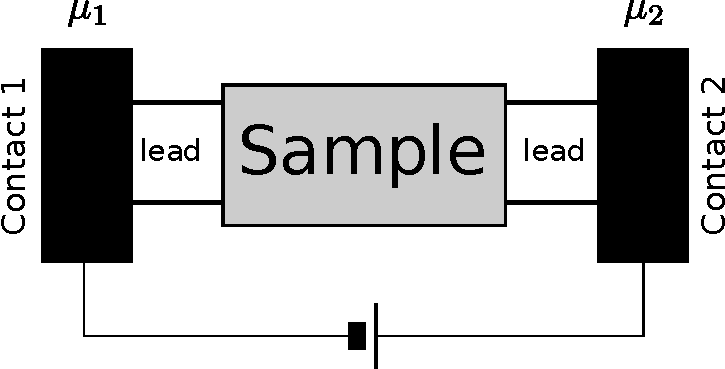
\includegraphics[width=0.5\textwidth]{sample-leads}
    \end{center}
    \caption{Schematic setup to derive the Landauer Formula}
    \label{fig:sample-leads}
\end{figure}

The sample is attached to two leads, which we assume to be perfect, ballistic
conductors with $M$ modes each. We assume that the contacts are
reflectionless, that is electrons can travel from the sample into the contacts
without reflection.

This means that the $k_x$ states in the left lead are occupied by electrons
coming from contact 1, and thus have the same electrochemical potential as
the contact, $\mu_1$. Likewise the $-k_x$ states in the right lead have the
potential $\mu_2$.

At zero temperature, only electrons with energies between $\mu_1$ and $\mu_2$
are transported, and the influx from the left lead is
$I_1^+ = (2e/h)M(\mu_1-\mu_2)$. We call the transmission probability through
the sample $T$, so the outflux from lead 2 is $I_2^+ = T I_1^+$, the rest
is reflected back: $I_1^- = (1-T) I_1^+$. The net current $I$ then is

\begin{align}
    I = I_1^+ - I_1^- = \frac{2e}{h} M T (\mu_1 - \mu_2)
\end{align}

The conductance is

\begin{align}
    G = \frac{I |e|}{\mu_1 - \mu_2} = \frac{2 e^2}{h} MT
\end{align}

\subsection*{Transmission and Green's functions}

To calculate the matrix $T$, one can make use of the so-called \emph{Green's
functions}. A Green's function $G$ is, loosely speaking, an inverse of a
differential operator $D$. More precisely if the relation between an
excitation $\delta$ and a response $R$ is $D R = \delta$, then every
operator $G$ for
which the equation $R = G \delta$ holds is called a Green's function.

To calculate the wave function $\psi$ in response to an excitation $\delta$ at a
given energy $E$ we can use the inhomogeneous Schrödinger Equation

\begin{align}
    \label{eq:green-define}
    (E - H) \psi = \delta
\end{align}

Where $H$ is the Hamiltonian operator. In a one-dimensional wire oriented
along the $x$ axis we expect an excitation of the form
$\delta = \delta(x - x_0)$ to result in two waves propagating away from $x_0$,
so our ansatz is

TODO: explicit form of $H$

\begin{align}
    G(x, x_0) = \begin{cases}
        A^+ e^{i k(x-x_0) } \qquad \textnormal{ for } x > x_0 \\
        A^- e^{-i k(x-x_0) } \qquad \textnormal{ for } x < x_0 \\
    \end{cases}
%    \left\{   \right.
\end{align}

This function satisfies Eqn. \ref{eq:green-define} for every point $x \not=
x_0$  for $ k = \sqrt{\frac{2mE}{\hbar^2}}$.

From the boundary conditions

\begin{align}
    G(x = x_0 + 0, x_0) - G(x = x_0 - 0, x_0) &= 0 \\
    \frac{\partial G(x, x_0)}{\partial x}\left.\right|_{x=x_0 +0}
    -\frac{\partial G(x, x_0)}{\partial x}\left.\right|_{x=x_0 -0}
        &= \frac{2m}{\hbar^2}
\end{align}

(where by $+0$ we mean \emph{evaluated from the right} and by $-0$ we mean
\emph{evaluated from the left}).

We obtain $A^+ = A^- = -\frac{i}{\hbar v}$ where $v := \frac{\hbar k}{m} $.

We call this particular solution the \emph{retarded Green's function} $G^R$,
to distinguish it from a second solution with opposite sign both in the $A$s
and in the exponent, which we call the \emph{advanced} Green's function $G^A$.

In a wire with finite width multiple modes can propagate, but since we can
separate the $x$ and $y$ components, the Green's functions become only
marginally more complex:

\begin{align}
    G^R(x, x_0) = \sum_m A^\pm_m \chi_m(y) e^{i k_m |x - x_0|}
\end{align}

where the transverse wave functions $\chi_m(y)$ satisfy the Schrödinger
Equation in $y$ direction with eigenvalue $\epsilon_m$.

Orthogonality of the different $\chi_m(y)$ functions and boundary conditions
give us an expression for the amplitudes:

\begin{align}
    A^\pm = - \frac{i}{\hbar v_m} \chi_m(y_0)
\end{align}

If $E$ is an eigenvalue of $H$, $(E-H)^{-1}$ does not exist. One guards
against such singularities by introducing a small, real number $\eta$ and
defines

\begin{align}
    G^R &= \left( (E + i \eta)\mathbf{1} - H \right)^{-1}\\
    G^A &= \left( (E - i \eta)\mathbf{1} - H \right)^{-1}
\end{align}

where $i$ is the complex unit.

One can (with some approximations) obtain a matrix representation for $H$
(see section \ref{sec:tight-binding}) and thus calculate the inverse, as
long as we only consider closed systems.

\begin{figure}
    \begin{center}
        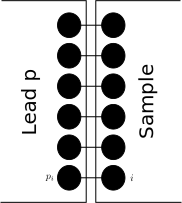
\includegraphics[height=5cm]{coupling-sample-lead}
    \end{center}
    \caption{Coupling between a lead and the sample}
    \label{fig:coupling-sample-lead}
\end{figure}

When we consider a discrete lattice both in the sample and in the leads, we
can couple adjacent lattice points in the sample and a lead as shown in Fig.
\ref{fig:coupling-sample-lead}.

The overall Green's function for both sample and lead can be partitioned into
a Green's function for the sample $G_s$, for the lead $G_p$ and two coupling
Green's functions $G_{sp}, G_{ps}$

\begin{align}
\left(
    \begin{array}{ll}
        G_p    & G_{ps}\\
        G_{sp} & G_s
    \end{array}
\right)
=
\left(
    \begin{array}{ll}
        (E + i\eta)\mathbf{1} - H_p   & \tau_p\\
        \tau_p^\dagger                & E\mathbf{1} - H_s
    \end{array}
\right)^{-1}
\label{eq:coupling-green}
\end{align}

Where $\tau_p$ is the coupling matrix for lead $p$, and contains only non-zero
entries $t$ for matrix elements connecting adjacent sites in lead and sample.

From \ref{eq:coupling-green} we can find an expression for $G_s$:

\begin{align}
    G_s = (E\mathbf1 - H_s - \tau^\dagger g_p^R \tau_p )^{-1}
\end{align}

Where $g_p^R$ is the retarded Green's function for the isolated lead $p$,

\begin{align}
    g_p^R = ((E+i\eta)\mathbf1 - H_p)^{-1}
\end{align}

$g_p^R$ can often be calculated analytically. We call the term $\tau^\dagger
g_p^R \tau_p$ \emph{self-energy} $\Sigma^R_p$. Its real part describes the
energy shift of an electron entering the sample, and the imaginary part
determines the life time of a state in the sample.

When multiple independent leads are attached
to the same sample, the effects of the self-energies for each lead simply add
up, and we get

\begin{align}
    G_s^R &= \left(E\mathbf1 - H_s - \sum_p \Sigma^R_p\right)^{-1} \\
    \textnormal{with } \Sigma^R_p &= \tau^\dagger g_p^R \tau_p
\end{align}

It can be shown \cite{fischer-lee,baranger} that the transmission $T_{pq}$ from lead
$q$ through the sample into lead $p$ is

\begin{align}
    T_{pq} = \trace(\Sigma_p G_s^R \Sigma_q G_s^A)
\end{align}

This is called the Fischer-Lee-Relation.

This allows numeric calculation of transmission coefficients for
arbitrary Hamiltonian operators, and is thus independent of the individual
phenomena we're looking at.

\subsection*{Rashba Spin-Orbit Coupling}

The Dirac equation from relativistic quantum theory describes an electron
coupled to a positron. Since the gap $\Delta = 2 m_e c^2$ is quite large, the
effect of the positron on the electron very small at low energies, and can be
taken into account by folding the $4\times4$ Hamiltonian (two dimension to
take spin into account, two for electron and positron) to an effective
$2\times 2$ Hamiltonian.

One of the terms in the Pauli equation resulting from this folding is the
\emph{Pauli Spin-Orbit coupling} term\cite{winkler2003}

\begin{align}
    \left( \ldots - \frac{e\hbar \vec\sigma \cdot \vec p \times \vec E}
                    {2\Delta} \ldots\right)\Psi = E \Psi
\end{align}

where $\vec E$ is the electric field and $\vec \sigma$ is the vector
which contains the Pauli matrices.

In solids the coupling takes place between holes and electrons. Since the
energy difference between the bands can be in the order of meV or eV
(as opposed to $\Delta \approx 1GeV$ for electrons in vacuum), the spin orbit
coupling strength can as much as one million times higher (TODO: citation)
than in vacuum.

In a solid in equilibrium any electric field is either part of the band
structure (and thus taken care of by folding down to a reduced Hamiltonian),
or is induced by a structural asymmetry.

In solid state physics the spin-orbit coupling term due to structural
inversion asymmetry is called \emph{Bychkov-Rashba} term or simply
\emph{Rashba} term (after \cite{rashba}), and is usually written as

\begin{align}
    H = \frac{\vec p ^2}{2m^*} + \alpha \inp{\vec I \times  \vec \sigma} \cdot \vec p
\end{align}

Where $\vec I$ is a unit vector pointing into the direction of the asymmetry,
$m^*$ is the effective mass
and $\alpha$ denotes the strength of the spin-orbit coupling.

This effect lifts the degeneracy of spin-up and spin-down electrons for
$k \not= 0$:

\begin{align}
    E(k) = \frac{\hbar^2}{2 m^*} k^2 \pm \alpha k
\end{align}
TODO: illustrative explanation.


\subsection*{Tight Binding Hamiltonian}
\label{sec:tight-binding}


In order to numerically evaluate the Green's function, we
discretize the sample into sites and assume that electrons only travel from
one site to an immediate neighbor. This allows us to represent the
Hamiltonian and other differential operators by a finite matrix.

% TODO: remove bullshit
% TODO: references
The nearest neighbor approximation is quite common in transport calculations,
and comes from the linear combination of atomic orbits (LCAO) ansatz, where
one assumes that the overlap between localized electron orbitals decreases
exponentially with distance.

In a two-dimensional square lattice the distance to the next nearest
neighbors is $\sqrt{2} a$ (where $a$ is the lattice constant), so one can
approximate that the overlap is $e^{-\sqrt{2}} \approx 0.24$. For a simulation
that tries to reproduce exact physical behavior of a sample one would have to
include the next-nearest neighbor hopping, and maybe even one further step
($e^{-2} \approx 0.14$).

But since our model is an effective one, we have to give up that claim
anyway, and instead ask ourselves if next-nearest neighbor hopping or higher
orders contribute any new physics, in terms of symmetries. To the best of our
knowledge that is not the case, so we keep the nearest neighbor approximation.

For a two-dimensional electron gas with Rashba spin-orbit coupling (of
strength $\alpha$) the Hamiltonian is

\begin{equation}
    H = \frac{1}{2 m^*} (p_x^2 + p_y^2) +
    \frac{\alpha}{\hbar} \inp{p_y\sigma_x - p_x\sigma_y}
\end{equation}

To map this to a discrete lattice we substitute the derivative by a discrete
difference, so $\dell_x f(x)|_{x_0}$ becomes $(f(x_0+a) - f(x_0))/a$. $a$ is
the lattice constant. For the
second derivative we chose the symmetric difference $\dell_x^2 f(x)_{x_0} =
(f(x_0+a) - f(x_0-a))/2a$. In the continuum limit $a \mapsto 0$ both reproduce
the derivative exactly.

Written in terms of creation and destruction operators we obtain

\begin{align}
    H   &= H_0 + H_r\\
    H_0 &= \sum_{n,\sigma} \epsilon_0 c^{\dagger}_{n\sigma} c_{n\sigma}
           - \sum_{n,\delta,\sigma} t c^\dagger_{n\sigma} c_{n,\sigma} +
           \textnormal{H.c.}\\
    H_r &= \frac{-\alpha}{2 a_0} \sum_m
        -i( c^\dagger_{m,\uparrow|} c_{m+a_y,\downarrow}
            + c^\dagger_{m,\downarrow} c_{m+a_y,\uparrow})
         + c^\dagger_{m,\uparrow|} c_{m+a_x,\downarrow}
            + c^\dagger_{m,\downarrow} c_{m+a_x,\uparrow}
\end{align}

where $n$ runs over all lattice sites, $\delta$ over $\uparrow$ and
$\downarrow$, and $a_x$ and $a_y$ denote the shift to the nearest neighbor in
$x$ and $y$ direction, respectively. (Note that we assume that the lattice is
equally spaced in $x$ and $y$ direction, $+a_x$ just means "go to the next
neighbor in $x$ direction"). $t = \frac{\hbar^2}{2ma}$ is the so-called hopping term, and denotes the
probability of an electron traveling to its nearest neighbor. $\tso$ is the
Rashba hopping term, and corresponds to a nearest neighbor hop with spin
flip.

Assume we have a quadratic system of $N \times N$ lattice sites.
For a two-dimensional system we enumerate all lattice sites row by row, and
use the result as the index to the Hamiltonian. To incorporate spin, we
identify the indexes that were assigned so far with spin-up, and add $N^2$ to
each index to obtain the matrix index for spin-down.

For example if our system were of size $3 \times 3$, the left-most site in the
first row has index $i = 1$, and the left-most site in the second row has
index $j = N + 1 = 4$ (both spin down). The interaction term (without spin
flip) between these two sites can thus be found at $H_{i,j} = H_{1,4}$. The
interaction that involves a spin flip from $\uparrow$ to $\downarrow$ is
described by $H_{i, j+N^2} = H_{1, 13}$.

\begin{figure}[tb]
    \begin{align*}
        H &= \inp{
           \begin{array}{cc}
                H_{kin}  & H_{spin} \\
                H_{spin}^\dagger & H_{kin} \\
           \end{array}} \\
           %
        H_{kin} &= \inp{
            \begin{array}{ccccccccc}
                -4t & t &  & t\\
                t & -4t & t &  & t &  &  & 0\\
                & t & -4t & 0 &  & t\\
                t &  & 0 & -4t & t &  & t\\
                & t &  & t & -4t & t &  & t\\
                &  & t &  & t & -4t & 0 &  & t\\
                &  &  & t &  & 0 & -4t & t\\
                & 0 &  &  & t &  & t & -4t & t\\
                &  &  &  &  & t &  & t & -4t\end{array}
        } \\
        %
        H_{spin} &= \inp{
            \begin{array}{ccccccccc}
                0 & -\tso &  & i\tso\\
                \tso & 0 & -\tso &  & i\tso &  &  & 0\\
                & \tso & 0 & 0 &  & i\tso\\
                -i\tso &  & 0 & 0 & -\tso &  & i\tso\\
                & -i\tso &  & \tso & 0 & -\tso &  & i\tso\\
                &  & -i\tso &  & \tso & 0 & 0 &  & i\tso\\
                &  &  & -i\tso &  & 0 & 0 & -\tso\\
                & 0 &  &  & -i\tso &  & \tso & 0 & -\tso\\
                &  &  &  &  & -i\tso &  & \tso & 0
            \end{array}
        }
    \end{align*}
    \caption{Tight binding Hamiltonian for $ 3 \times 3 $ lattice sites}
    \label{fig:hamiltonian}
\end{figure}

Figure \ref{fig:hamiltonian} shows an example Hamiltonian for a system of
$3 \times 3$ lattice sites with Rashba spin-orbit coupling (and no magnetic
field).

Sites at the edge of the sample have no hopping element to a neighboring site
at the outside of the sample, so we have hard wall boundary conditions. All
interaction with the outside world is modeled through the self-energy induced
by the attached leads.

\NeedsTeXFormat{LaTeX2e}
\documentclass[11pt]{article}
%Absaetze nicht einruecken:
\usepackage{parskip}
\usepackage[utf8]{inputenc}
\usepackage[T1]{fontenc}
\usepackage{ae}
\usepackage[intlimits, sumlimits, namelimits]{amsmath}
\usepackage{bbm}
%Neue Macros fuer Mathe:
%in parentheses - gleich mit richtiger Groesse
\newcommand{\inp}[1]{\ensuremath{\left(#1\right)}}
\newcommand{\sqr}{\ensuremath{^{2}}}
\newcommand{\cube}{\ensuremath{^{3}}}
%Mengensymbole mit doppelten senkrechten Strichen:
\newcommand{\set}[1]{\ensuremath{\mathbbm{#1}}}
%definiert eine Norm, also zwei senkrechte Striche auf jeder Seite:
\newcommand{\norm}[1]{\ensuremath{\left|#1\right|}}
\newcommand{\vect}[2]{\ensuremath{\inp{\hspace{-.8ex}\begin{array}{c}#1\\#2\end{array}\hspace{-.4ex}}}}
%\newcommand{\vec3}[3]{\ensuremath{\inp{\hspace{-.8ex}\begin{array}{r}#1\\#2\\#3\end{array}\hspace{-.4ex}}}}
\newcommand{\entspr}{\ensuremath{\,\,\hat{=}\,\,}}%
\newcommand{\dx}[1][x]{\ensuremath{\textnormal d #1}}

\newcommand{\ta}{\tilde \alpha}

% For stupid thinkos:
\newcommand{\cross}{\times}

% Tabellen:
\usepackage{array}
\setlength{\extrarowheight}{.2mm}
%Links im Text:
\usepackage{hyperref}
\usepackage{graphics,graphicx,fancyvrb}
%Raender einstellen
%\usepackage[a4paper, left=25mm, right=5mm, top=30mm]{geometry}
\usepackage[a4paper]{geometry}
%Kopf - und Fusszeilen
\usepackage{lastpage}
\usepackage{fancyhdr}
	\lhead{Moritz Lenz}
	\chead{\bfseries{-- \thepage\ --}}
	\rhead{\thetitle}
	\lfoot{}
	\rfoot{}
	\cfoot{}
	\pagestyle{fancy}
\pagestyle{empty}

\sffamily

%Kopfzeile

\author{Moritz Lenz}
\title{Spintronics}
\begin{document}
\maketitle

This is an attempt to reproduce what Khodas wrote in {\em Spin 
Polarization of Nonmagnetic Heterostructures: The Basics of Spin
Optics}, PRL 92.086602.

The setup consists of a 2D electron gas in the $x-z$ plane, where the
strength of the spin orbit interaction is a step function in $x$:
$\alpha(x) = \alpha \Theta(x)$. The region $x < 0$ is called the
"normal region", abbreviated with N, and the region with $x > 0$ is
called the "spin orbit" region, abbreviated as SO.

The Hamiltonian looks like this:

\begin{align}
    H_r &= \frac{p^2}{2m} + (-\vec y \times \vec \sigma) \cdot
            \alpha(x) \vec p\\ 
    p^2 &= p_x^2 + p_z^2
\end{align}

With the eigenvalues and the velocities

\begin{align}
    E_{\pm} &= \frac{p^2}{2m} \pm \alpha \\
    v_{\pm} &= \frac{\partial E_{\pm}}{\partial p} = \frac{p}{m} \pm \alpha
\end{align}

When a wave travels from the N to the SO region it's energy doesn't
change. Since its dispersion relation changes, the momentum must also
change. From here on when we write $p$ we mean the momentum in the N
region. The momentum in the SO region then follows as

\begin{align}
    \label{eq:pso}
    p_{SO}^{\pm} &= m v_F (\sqrt{1 + \ta^2} \mp \tilde \alpha) \\
    \tilde\alpha &= \frac{\alpha}{v_F}
\end{align}

$p_z$ is conserved at the interface.

Solving the eigenvalue equation leads us to the eigenvectors in the SO
region:

\begin{align*}
   \chi_{SO}^{\pm} &= \frac{1}{n_{SO}^{\pm}} 
                      \vect{-p_{x,SO}^{\pm} \pm p_{SO}^\pm}{p_z} \\
    (n_{SO}^{\pm})^2 &= (-p_{x,SO}^{\pm} \pm p_{SO}^\pm)^2 + p_z^2
\end{align*}

Where the lower index $x$ means that the value is projected onto the
$x$ axis. The angle between the $x$ axis and the momentum of the
incident wave is called $\phi$, so that $p_x = p \cos \phi$.

Note that in the N regime $H$ is a diagonal matrix, and the direction
of the eigenvectors can be chosen with some freedom. We pick
$\chi_N^{\pm} = \lim_{\alpha \mapsto 0} \chi_{SO}^{\pm}$ to ensure that
$<\chi_N^+|\chi_{SO}^+> = 1$ holds true at a vanishing interface.



The overall wave function consists of an incident wave, 
and reflected and transmitted part. In general the incident wave can
be decomposed into one with $+$ and one with $-$ chirality, which
propagate and scatter independently. Let's consider the incident $+$
wave:

\begin{align}
    \Psi^+ = e^{i p_z z} * \left\{
        \begin{array}{ll}
            e^{i p_x x} \chi_N^+ + e^{- i p_x x} (\chi_N^+ r_{++} +
                    \chi_N^- r_{-+})    & x < 0\\
            e^{i p_x^+ x} \chi_{SO}^+ t_{++} + e^{i p_x^- x}
            \chi_{SO}^- t_{-+}          & x > 0
        \end{array} \right.
\end{align}

The coefficient $r_{-+}$ is the amplitude with which the incident wave
of $+$ chirality is reflected into $-$ chirality etc. while $t$
coefficients stand for transmission coefficients.

Analog equations can be found for the incident wave with $-$ chirality
by changing all signs that appear either as a subscript or
superscript.

To obtain the values for these coefficients one has to solve the
boundary conditions at the interface. The wave function is continuous
and the current is conserved, so $\frac{\partial H}{p_x} \Psi$ is also
continuous.

\begin{align}
    \Psi_N|_{x = -0}    &= \Psi_{SO}|_{x = +0} \label{eq:continuous}\\
    \left.\frac{\hat p_x}{m} \Psi_N\right|_{x = -0}
                        &= \left. \left(\frac{\hat p_x}{m} -\alpha \sigma_z\right)
                                \Psi_{SO}\right|_{x = +0}
\end{align}

The second equation can be evaluated with $\hat p_x = -i \partial_x$
(assuming $\hbar = 1$, as done in the rest of the calculation) and
carrying out the derivation (and multiplied by $m$), yielding

\begin{align}
    p_x \chi_N^+ (1 - r_{++}) - p_x \chi_N^- r_{-+}
        =& p_x^+ \chi_{SO}^+ t_{++} + p_x^- \chi_{SO}^- t_{-+} \nonumber\\
         &   - m \alpha \left(  \sigma_z \chi_{SO}^+ t_{++}
                            + \sigma_z \chi_{SO}^- t_{-+} \right)
\end{align}

Dividing it by  $p_x = p \cos \phi$: 

\begin{align}
    \chi_N^+ (1 - r_{++}) - \chi_N^- r_{-+}
        =& \frac{p_x^+}{p_x} \chi_{SO}^+ t_{++} + \frac{p_x^-}{p_x} \chi_{SO}^- t_{-+} \nonumber\\
         &   - \frac{\ta}{\cos \phi} \left(\sigma_z \chi_{SO}^+
                 t_{++} + \sigma_z \chi_{SO}^- t_{-+} \right)
                                \label{eq:j_continuous}
\end{align}

Equations \ref{eq:continuous} and \ref{eq:j_continuous} can be
expanded in powers of $\ta$. In solutions expanded to the first
non-zero order each are

\begin{align}
    t_{++} &= 1 +
            \frac{\ta}{2}\left( \frac{1}{\cos^2\phi} - 1 \right)\\
    t_{-+} &= \frac{\ta^2}{4}\tan \phi \\
    r_{++} &= \frac{\ta}{2} \tan^2 \phi\\
    r_{-+} &= -\frac{\ta}{2} \tan \phi
\end{align}

And for the incident wave with $-$ chirality

\begin{align}
    t_{--} &= 1 - \frac{\ta}{2} \left( \frac{1}{\cos^2\phi} - 1 \right)\\
    t_{+-} &= O(\ta^3)\\
    r_{--} &= -\frac{\ta}{2} \tan^2 \phi\\
    r_{+-} &= -\frac{\ta}{2} \tan \phi
\end{align}

%and $n_{N}^\pm = n_{SO}^\pm$. With $n_N^- / n_N^+ = \tan
%\frac{\phi}{2}$ 

%
%Multiplying both equations with $\chi_N^+$ and $\chi_N^-$ gives us
%four scalar equations:
%
%\begin{align} 
%    \label{eq:a1}
%    1 + r_{++}  =& <\chi_{SO}^+|\chi_N^+> t_{++} +
%                    <\chi_{SO}^-|\chi_N^+> t_{-+}\\
%    \label{eq:a2}
%        r_{-+}  =& <\chi_{SO}^+|\chi_N^-> t_{++} + <\chi_{SO}^-|\chi_N^-> t_{-+}\\
%    \label{eq:b1}
%    1 - r_{++}
%        =& \frac{p_x^+}{p_x} <\chi_N^+|\chi_{SO}^+> t_{++}
%           + \frac{p_x^-}{p_x} <\chi_N^+|\chi_{SO}^-> t_{-+} \nonumber\\
%         &   - \frac{\ta}{\cos \phi} \left(
%                 <\chi_N^+|\sigma_z|\chi_{SO}^+> t_{++}
%                 + <\chi_N^+|\sigma_z|\chi_{SO}^-> t_{-+} \right)\\
%    \label{eq:b2}
%    -r_{-+}
%        =& \frac{p_x^+}{p_x} <\chi_N^-|\chi_{SO}^+> t_{++}
%           + \frac{p_x^-}{p_x} <\chi_N^-|\chi_{SO}^-> t_{-+} \nonumber\\
%         &   - \frac{\ta}{\cos \phi} \left(
%                 <\chi_N^-|\sigma_z|\chi_{SO}^+> t_{++}
%                 + <\chi_N^-|\sigma_z|\chi_{SO}^-> t_{-+} \right)
%\end{align}
%
%(The scalar products of the spinors are indicated in bracket notation
%for clarity, even though they don't imply an integration over any
%variable).

%Using the geometric relations
%
%\begin{align}
%    p^2         &= p_z^2 + p_x^2\\
%    p_{SO}^2    &= p_z^2 + p_{x,SO}^2
%\end{align}
%
%together with eqn. \ref{eq:pso} we have all quantities to calculate
%the scalar products.
%
%we have the means to solve these equations. 

\end{document}

% vim: ts=4 sw=4 expandtab spell spelllang=en_us tw=70

\chapter{Numerical Calculations}

Numerical transport calculations have a huge advantage over the analytical
calculation: once a formalism is implemented, it works for arbitrary
configurations within the limits of the model. However, it does not generally
supply us with data that enhances physical understanding, so it is best use as a
means to expand on analytical calculations which we already understand.

In that spirit we performed numeric calculations, simulating a sample with
Rashba Spin-orbit coupling, and spin-resolved leads attached at the edges.

The calculation follows this rough scheme:

\begin{itemize}
    \item set up the Hamiltonian $H$
    \item calculate the self-energy matrices $\Sigma_p$
    \item calculate the Green's functions $G^A$ and $G^R$ by inverting
          $H + \sum_p \Sigma_p$
    \item use the Fisher-Lee relation to calculate the transmission matrix $T$
            from $G^R$, $G^A$ and $\Sigma_p$
\end{itemize}

\section{Performance Consideration}

These numeric calculations are computationally expensive. If we simulate a
lattice with a total of $n \times n$ sites, the matrices $H$, $\Sigma_p$, $G^R$ and
$G^A$ are of dimensions $2n^2 \times 2n^2$. Inversion of an $m \times m $
matrix and multiplication of two $ m \times m $ matrices, both take $O(m^3)$
steps\footnote{There are matrix product algorithms with slightly better
asymptotic scaling, but they are usually very complicated, numerically badly
conditioned or only advantageous for huge systems; usually all three apply}
\cite{matrixperformance}. All other steps are faster and can be ignored for
an asymptotic analysis.

So the naive approach takes $O(n^6)$ steps for $n \times n$ lattice sites.

An alternative approach, the \emph{Recursive Green's Function method} works by
decomposing the sample into slices in such a way that the sites in each slice
only interact with neighbor slices. For short range interactions such a
decomposition can be found, and for nearest-neighbor hopping the time
complexity approaches $O(n^3)$ \cite{rgfschmelcher}. However, this is payed by
a significantly increased implementation complexity, and the algorithm is tied
to the specific form of the Hamiltonian.

\begin{figure}[htb]
    \begin{center}
    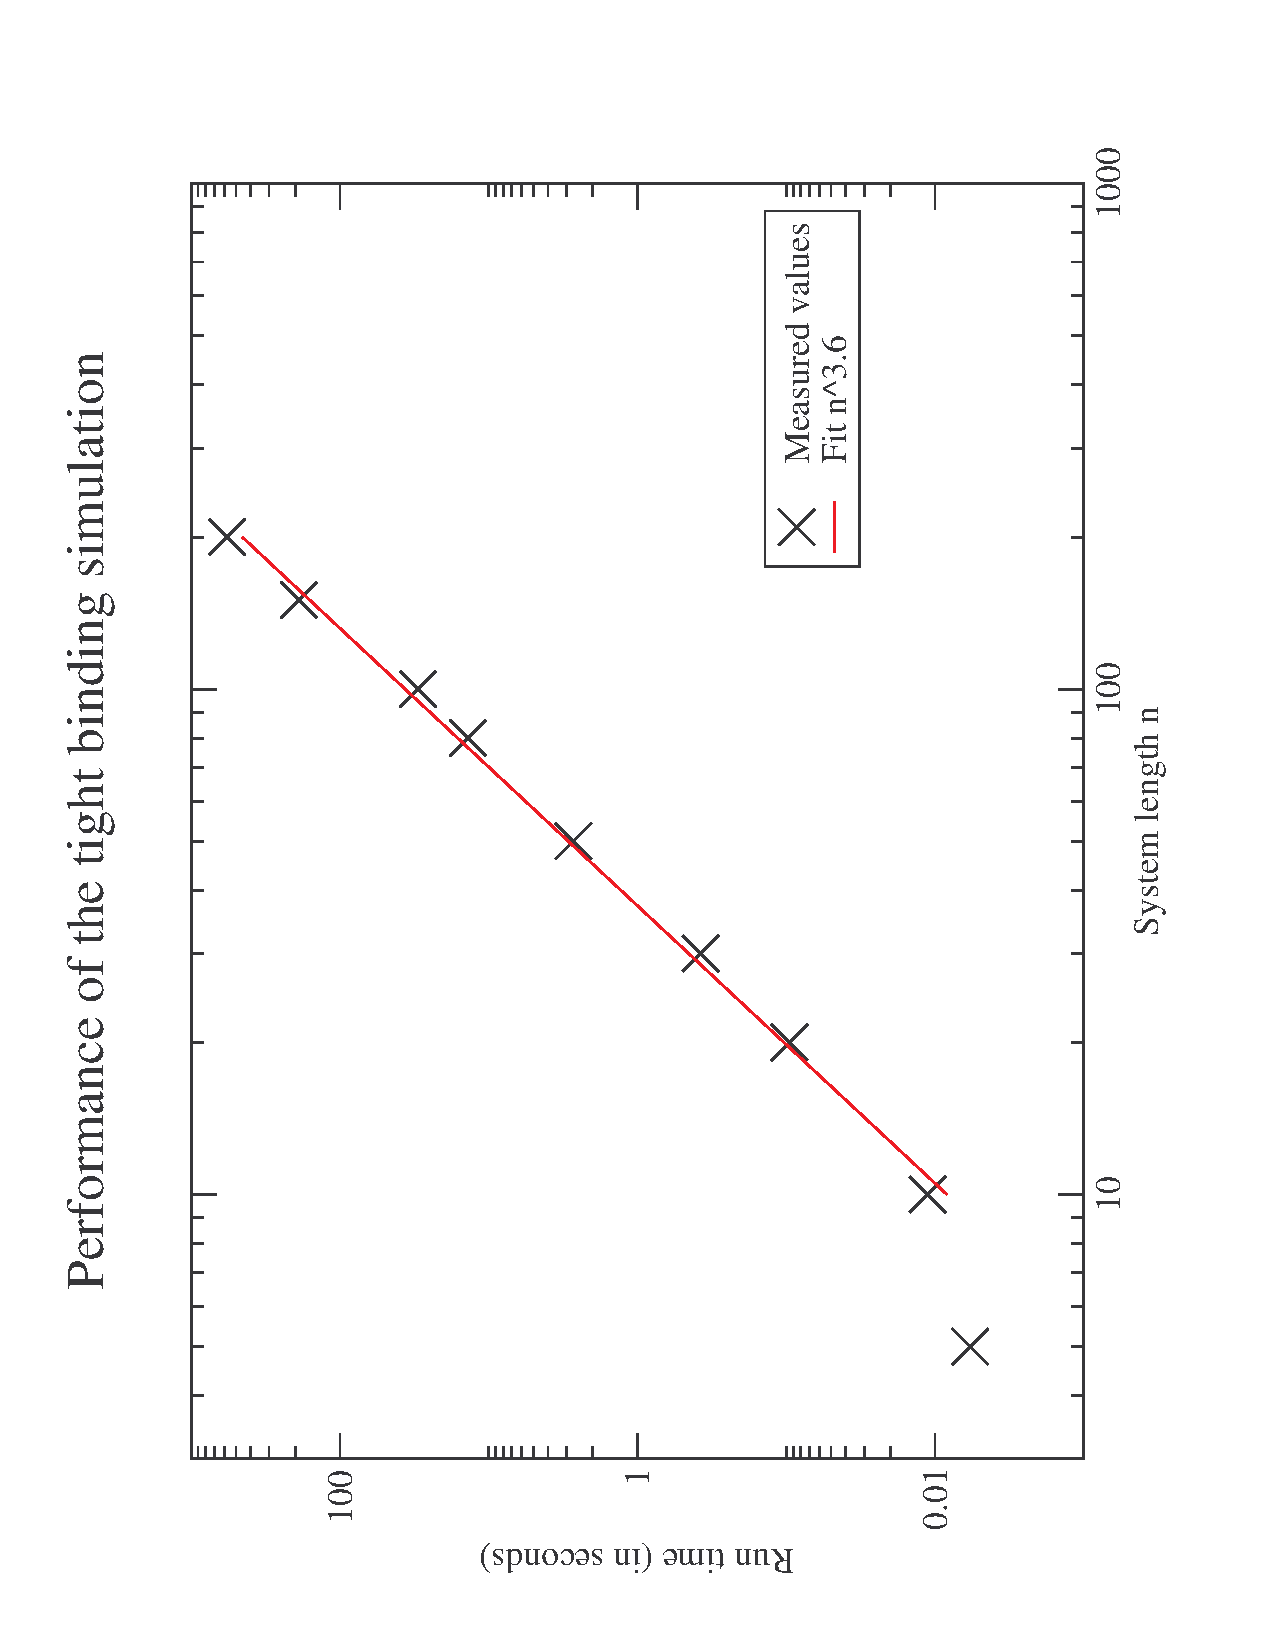
\includegraphics[angle=270,width=0.7\textwidth]{scaling.pdf}
    \end{center}
    \caption{Scaling of run time with system size for the tight binding
        simulation, implemented with sparse matrices and the SuperLU sparse
        direct solver. The data was recorded for square samples including
        Rashba spin-orbit coupling and 4 leads of the same width as the
        sample, on a 2.9GHz AMD64 computer with SSE2 and 8GB RAM.
        The run time approximately scales as $t(n) = 2
        n^{3.64}\mu s$}
        \label{fig:scaling}
\end{figure}

We chose a middle ground: the "naive" approach, but implemented with sparse
matrices and an efficient sparse direct solver \cite{superlu99} for
computing the Green's functions.

The run time thus depends largely on the number of non-zeros in the $H$ and
$\Sigma_p$ and thus on the nature of the interaction. For nearest neighbor
hopping and Rashba spin-orbit coupling, we observed a run time scaling of
$O(n^{3.64})$ (See Fig. \ref{fig:scaling}).

\section{Numerical Stability}

The numerical
calculation uses floating point numbers with limited machine precision,
therefore numerical errors are inevitable.

The transmission matrix for a sample, which is connected to multiple uniform
leads (with same number of modes per lead), has to fulfill the sum rules

\begin{align}
    \sum_p T_{pq} = \sum_q T_{pq} = M
    \label{eq:sumrule}
\end{align}

where $M$ is the number of modes (and thusly and integer). We can calculate
this left hand side of this equation from the numerical simulation, round it
to the nearest integer and thus estimate the numerical error in $T_{pq}$.

Since generally matrix inversion is numerically worse conditioned than solving
a linear equation system \cite{matrixinversion}, we do not actually compute
$G^A$ and $G^R$, but rather the products $G^A\Sigma_p$ and $G^R\Sigma_q$,
which can be written as solutions of linear equation systems.

\begin{align}
    X_p &= \Sigma_p G^R\\
    X_p^\dagger &= (G^R)^\dagger \Sigma_p^\dagger = G^A \sigma_p^\dagger\\
    \Rightarrow\quad (G^A)^-1 X_p^\dagger &= \Sigma_p^\dagger
    \label{eq:lin_gls}
\end{align}

Eq. \ref{eq:lin_gls} is the form with which linear sparse solvers typically
work. They usually calculate a LU decomposition (they write
$(G^A)^-1 = L \cdot U$, where $L$ is a lower triangular matrix and $U$ an
upper triangular matrix), and directly solve the equation by elimination.
Complex conjugation and transposition of $X_p^\dagger$ finally gives us the
matrix which we need evaluating the Fischer-Lee relation.

\begin{figure}[htb]
    \begin{center}
    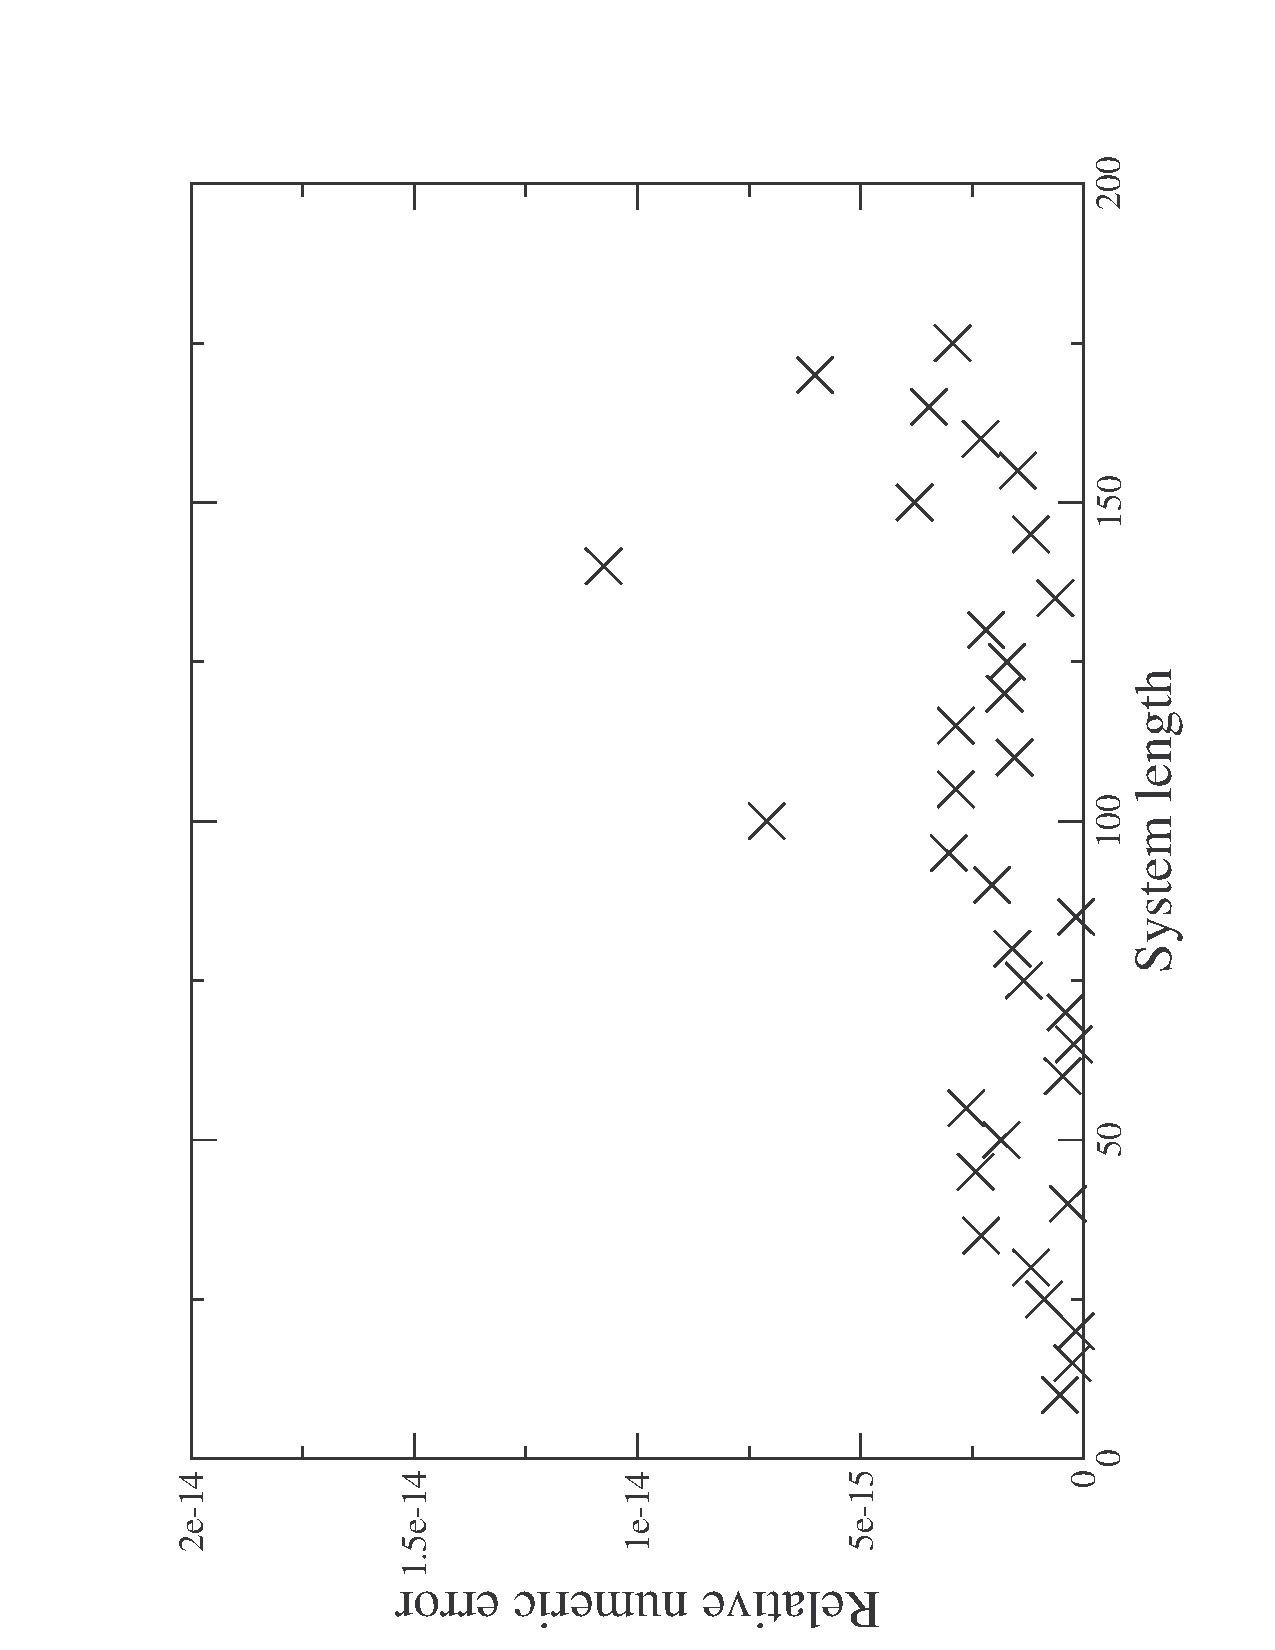
\includegraphics[angle=270,width=0.8\textwidth]{numeric-errors.pdf}
    \end{center}
    \caption{Numerical errors in $T_{pq}$ as a function of system size.}
    \label{fig:numeric-errors}
\end{figure}

Fig. \ref{fig:numeric-errors} shows the estimate of the numerical errors, and
that they are well below $10^{-13}$ for the investigated systems and
thusly are no source for worries.

\section{Quality Checks}

Programming is constantly prone to subtle errors, so measures had to 
be taken to ensure that no errors slipped in that might lead to wrong
output.

The program we discussed herein is basically a function that constructs a
Hamilton operator from the Rashba coupling strength, magnetic
field and other parameters, and then calculates the transmission
matrix $T_{pq}$ from that Hamilton operator.

The very first sanity check is that $H$ is indeed a hermitian
operator. This check, of course, only catches stupid programming
mistakes.

A more elaborate check is that $T_{pq}$ obeys the same symmetries as
the Hamiltonian. Since it can be written as
  
\begin{equation}
H = \frac{\vec{p}^2}{2 m^*} + \vec \sigma \cdot (\vec e_z \times \vec p)  
    + \vec \sigma \cdot \vec B
\end{equation}

it is easy to see that $H(\vec p, \vec \sigma, \vec B) = H(-\vec p,
-\vec \sigma, -\vec B)$, so the transmission matrix must follow the
same symmetries.

We checked these symmetries and the sum rule (eq. \ref{eq:sumrule}) regularly
to ensure that no simple errors slipped in.

\section{Convergence}
\begin{figure}[htb]
    \begin{center}
        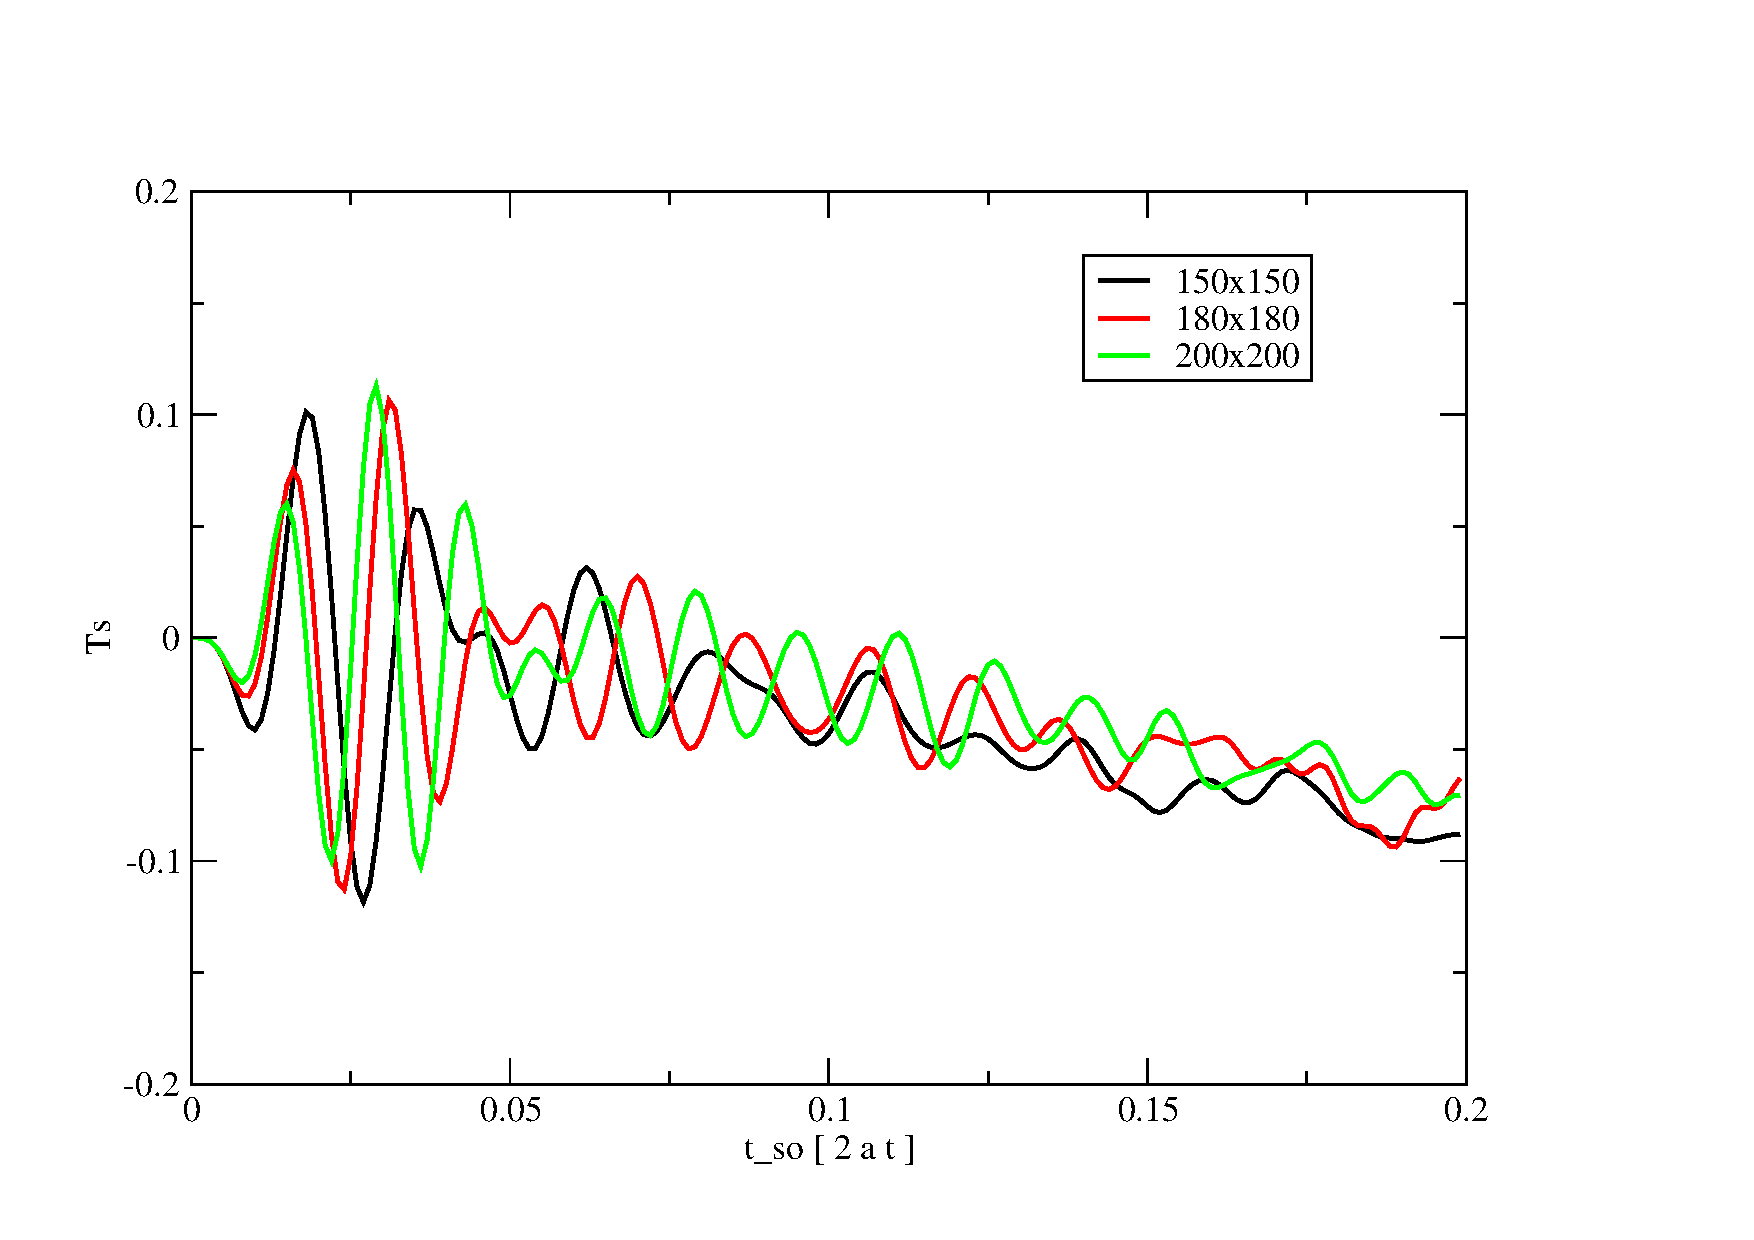
\includegraphics[width=0.8\textwidth]{convergence.pdf}
    \end{center}
    \caption{$T_S = T_{2\uparrow,1\uparrow}-T_{2\downarrow,1\downarrow}$ as a
        function of spin-orbit coupling strength for the setup described in
        section \ref{sec:numeric-setup} with different number of lattice
        sites.}
    \label{fig:convergence}
\end{figure}

The tight binding model is only exactly valid in the limit $ a \mapsto 0$,
i.e. vanishingly small lattice constant. Since the simulation requires a finite
$a$, we have to ensure that the $a$ is actually small enough to not make much
of a difference. This can be done by choosing a smaller $a$ for comparison.

Figure \ref{fig:convergence} shows this for a sample of $100~nm \times 100~nm$.
The results for the resolutions $150 \times 150$, $180 \times 180$ and $200
\times 200$ looks quite similar, but not quite identical. This is because, for
the larger resolution, more modes propagate. Still the qualitative behavior is
sufficiently similar to warrant the use of a $150 \times 150$ grid in the
following simulations.

\section{Setup}
\label{sec:numeric-setup}

\begin{figure}[htb]
    \begin{center}
        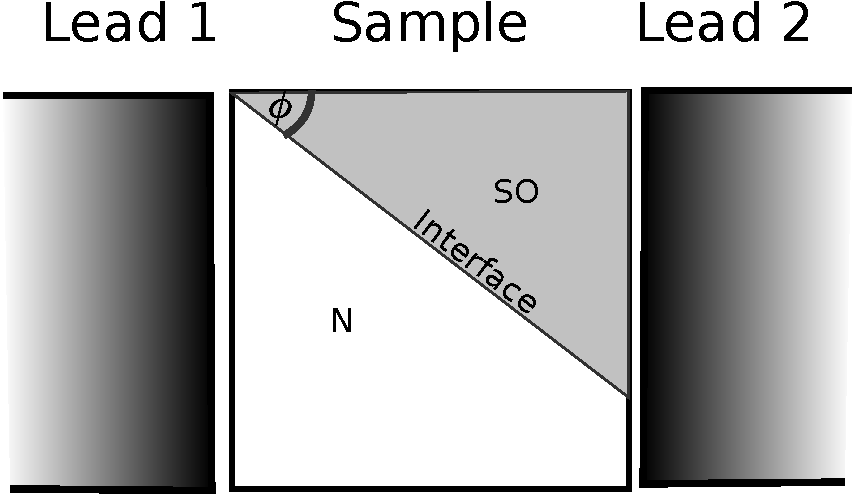
\includegraphics[width=0.5\textwidth]{sample-lead-interface.pdf}%
        \hspace{0.1\textwidth}%
        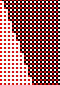
\includegraphics[width=0.2\textwidth]{hopping.png}
    \end{center}
    \caption{\textbf{Left:} The sample is connected to one lead for each spin
        on the left and on the right.
        \textbf{Right:}
        Detail from an interface between normal and spin-orbit coupling regime modeled
        in the tight binding model, at angle $\phi = 70\,^{\circ}$.
        Red dots show lattice sites, black dots
        show non-zero hopping elements with spin flips.}
    \label{fig:interface-setup}
\end{figure}

For the following simulations, we used a square sample, typically of $150
\times 150$ lattice sites, with two leads attached both on the left and on the
right, one for spin up, one for spin down.

\section{Interfaces at Arbitrary Angles}

To simulate an interface of an arbitrary angle $\phi$, we calculate the Rashba
hopping elements separately for each lattice site and install them for
hopping to the right and upper neighbor each. Fig. \ref{fig:interface-setup}
shows how such an interface looks.

\begin{figure}[htb]
    \begin{center}
        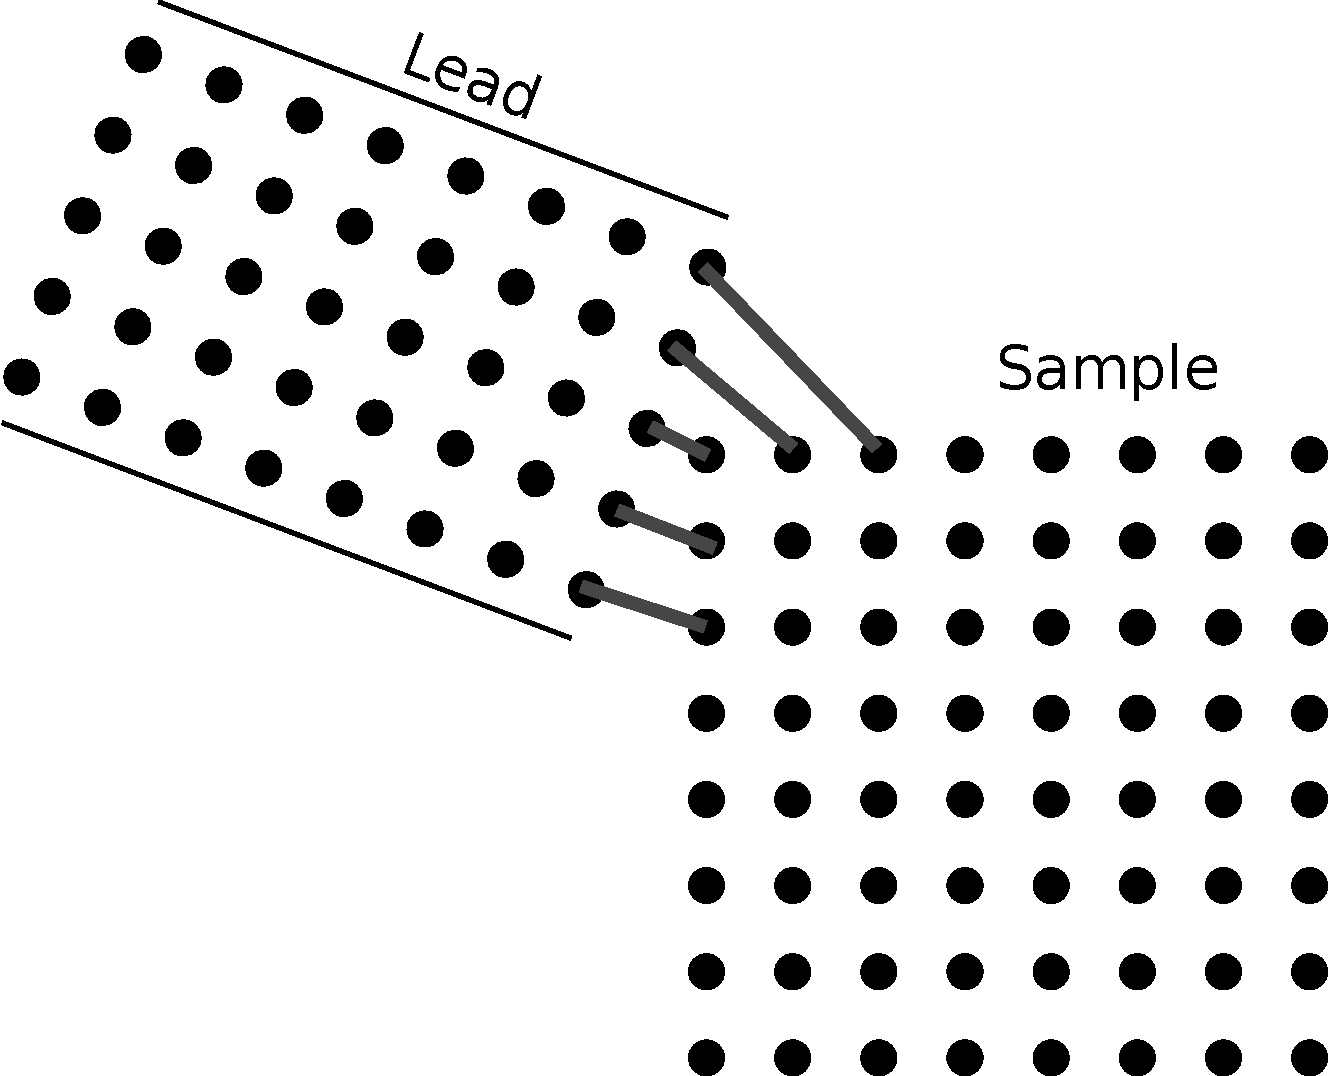
\includegraphics[width=0.4\textwidth]{lead-tilted-1.pdf}
        \hspace{0.1\textwidth}
        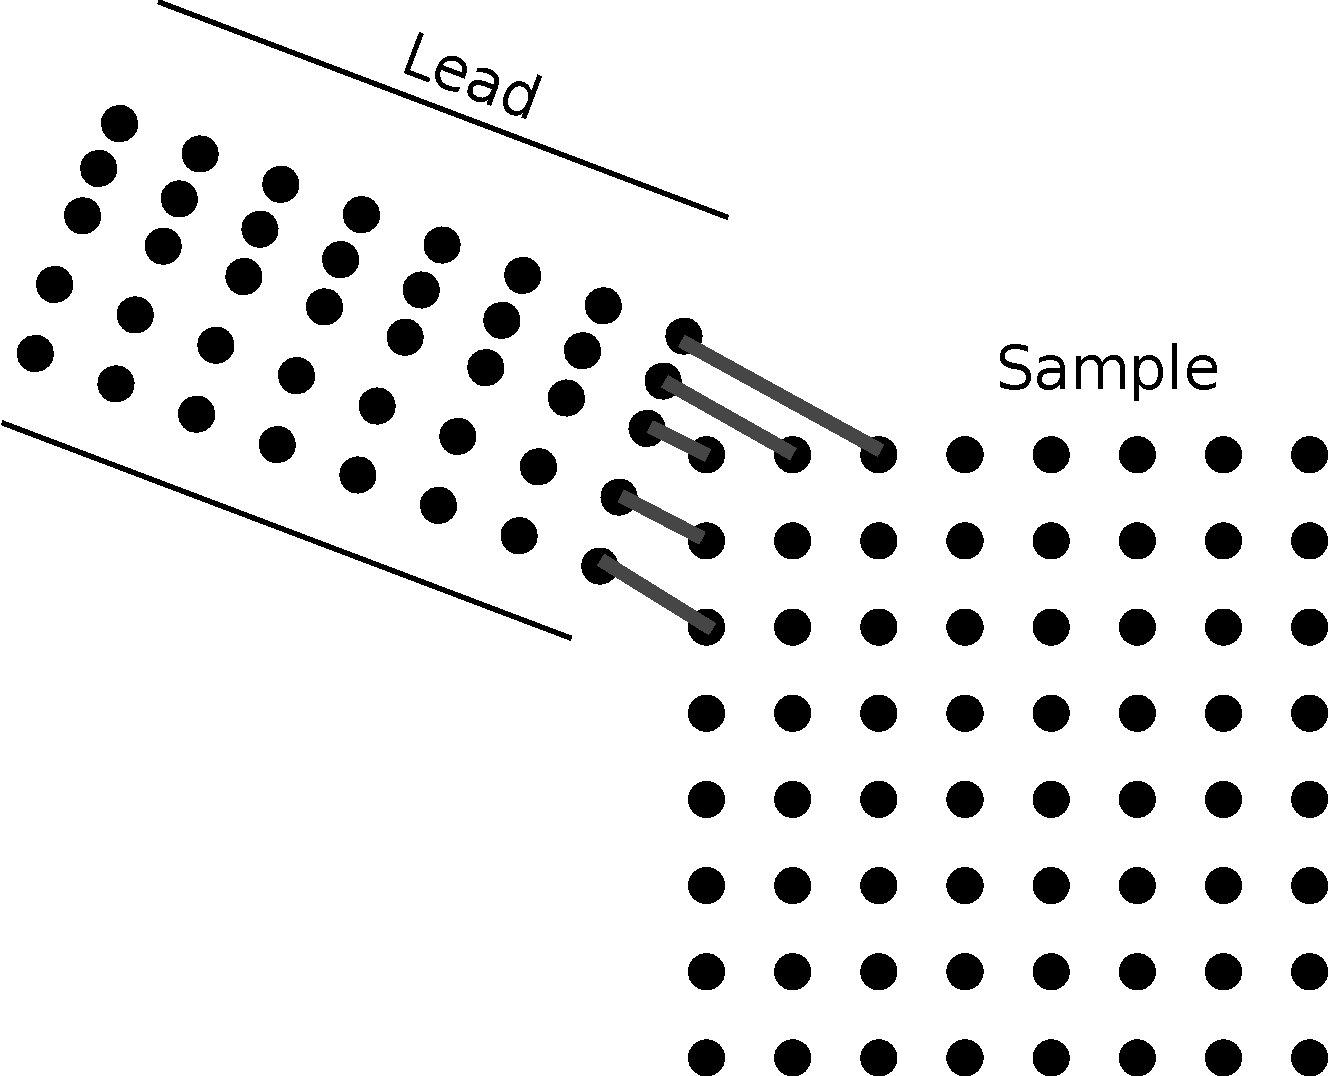
\includegraphics[width=0.4\textwidth]{lead-tilted-2.pdf}
    \end{center}
    \caption{Two ways to attach a tilted lead. \textbf{Left:} Equal lattice
        spacing in lead and sample. \textbf{Right:} Parallel projection from
        the sample into the lead leads to uneven lattice spacing in the lead.}
    \label{fig:tilted-leads}
\end{figure}

To obtain a smoother interface, we also experimented with using a vertical
interface, and injecting the electron beam with a defined angle through a tilted lead.

There are two possible
ways to do this (as illustrated by figure \ref{fig:tilted-leads}):
either one can assume the same lattice spacing in lead and sample and assume
coupling even though the geometry does not match, or one can project the sites
from the edge of the sample parallel into the lead and then get a non-regular
lattice spacing in the lead.

The former turned out not to work the way we wanted it to: instead of one
electron beam propagating in the same direction as the lead, there were two
beams, one parallel to each side of the edge of the sample. The latter is
physically hard to interpret and also much effort to implemented, so we set
that idea aside.

\section{Interface Between Normal and Spin-Orbit Coupling Region}

\begin{figure}[htb]
    \begin{center}
    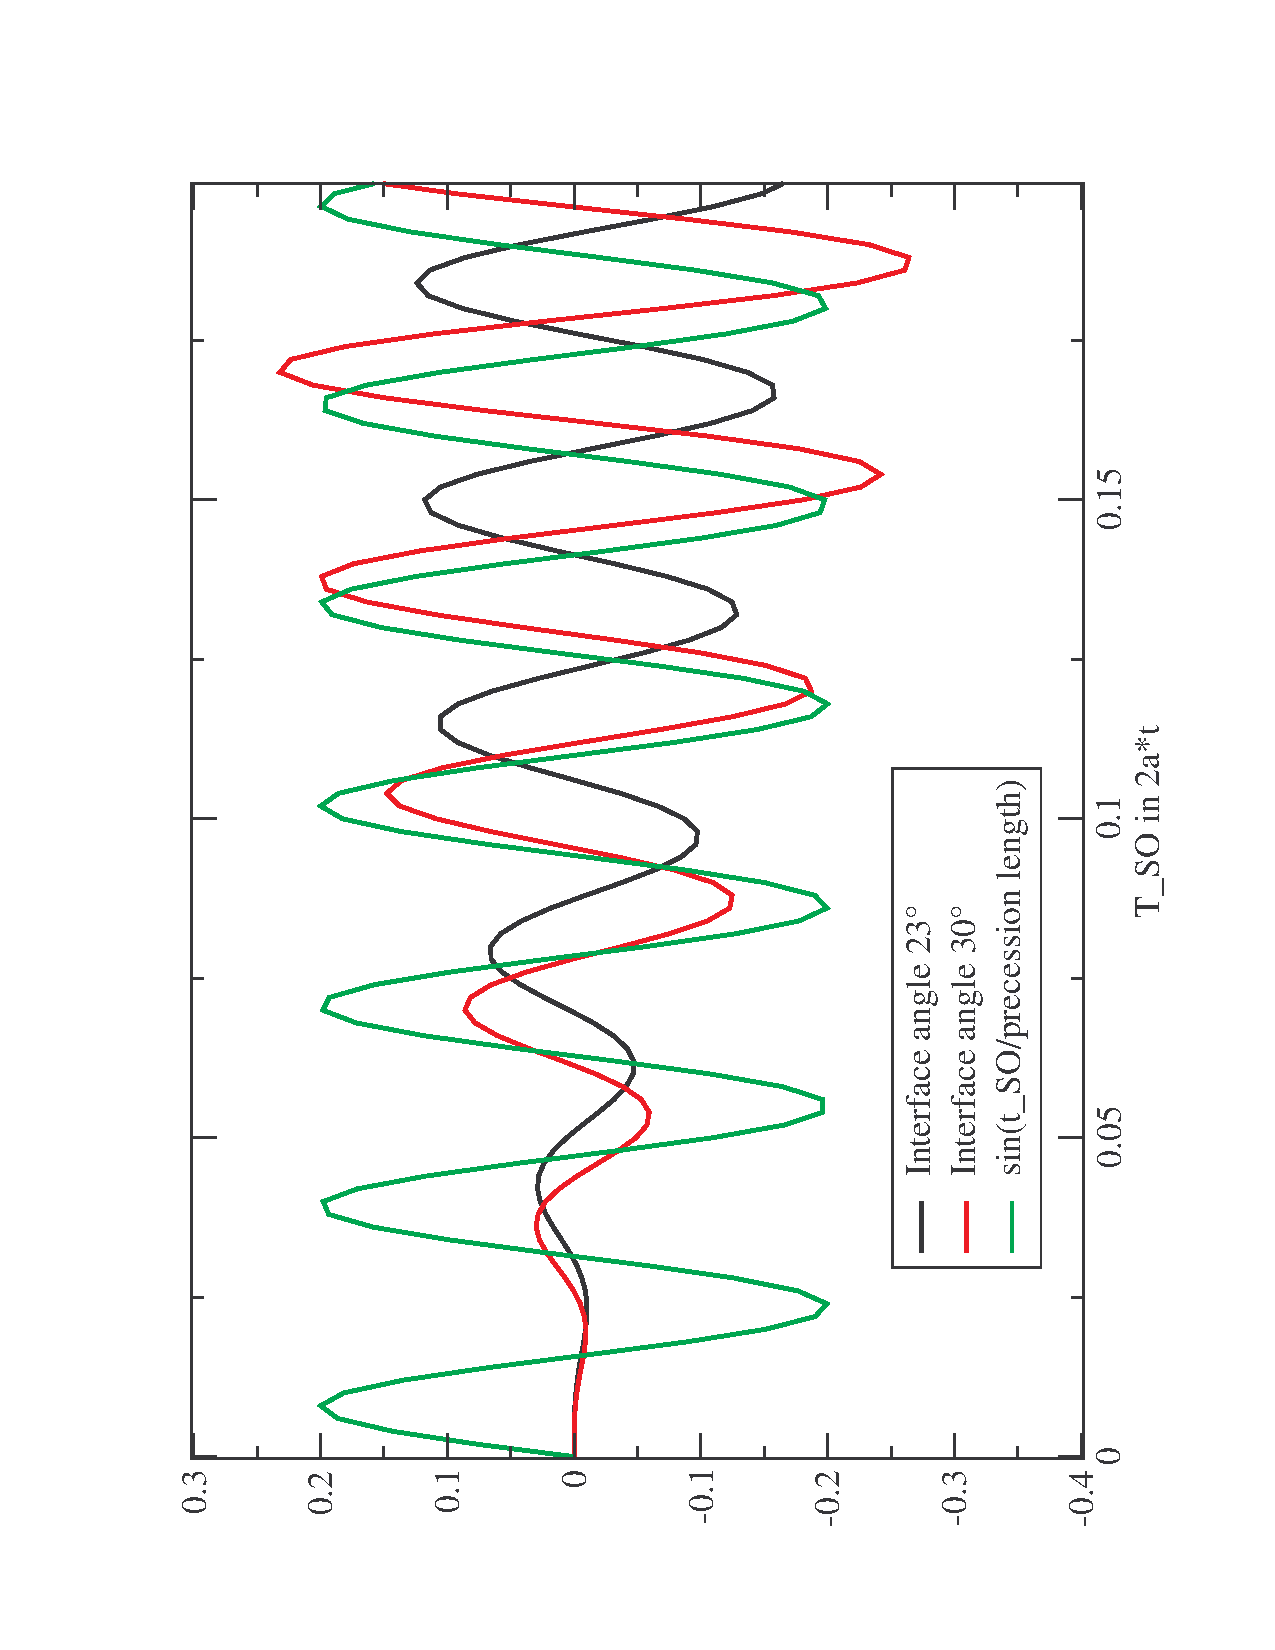
\includegraphics[angle=270,width=0.7\textwidth]{interface-precession.pdf}
    \end{center}
    \caption{$T_S = T_{2\uparrow,1\uparrow}-T_{2\downarrow,1\downarrow}$ as a
        function of spin orbit coupling strength. The interface causes a
        separation of spins which oscillates and is dependent on the angle of
        the interface.}
    \label{fig:interface-precession}
\end{figure}

When plotting $T_S = T_{2\uparrow,1\uparrow}-T_{2\downarrow,1\downarrow}$ as a
function of spin orbit coupling strength, one sees that the signal oscillates
(see figure \ref{fig:interface-precession}).
This is caused by the well-known % TODO: cite
spin precession: in a medium with spin-orbit coupling, $\sigma_z$ is not a good
quantum number anymore, and the spin precesses. % around what?

So if an electron is injected with spin up,and is measured after the
precession length $\lso = \frac{t}{\tso}\pi a$, it is again found to have
spin up, but, after $\frac12 \lso$ or $\frac32 \lso$, the spin points
downwards. 

Since  $\lso$ is a function of $\tso$, the precession can also be
observed when $\tso$ is varied (and not the width of the sample).
If $n$ is an integer and $W$ the width of our sample, we should see the
same signal for $W = n \cdot \lso(n)$ and $W = (n+1) \lso(n+1)$. So
$\tso(n) = n\frac{\pi t}{W}$ and $\Delta \tso = \frac{\pi t}{W}$.  The green
curve in figure \ref{fig:interface-precession} shows the curve
$\sin{\frac{2 \pi \tso}{\Delta \tso}}$ and thus the expected spin precession.

Only a part of the sample has non-zero spin-orbit coupling strength, so $T_S$
actually precesses with a slightly longer period than $\Delta \tso$.

\subsection{Comparison to Analytical Results}

The chiral spin bases as introduced in chapter \ref{sec:analytical} are very
natural for the analytical calculation, because the
base vectors are also eigenstates to the Hamiltonian.

One might think that the easiest way to compare analytical and numerical
results is to simply use the chiral bases in the leads, but that is a
misconception. The chiral spin bases depend on the real space direction
of the waves, and, in the SO regime thus not known a priori --
rather it is an intermediate
result of the numerical calculation\footnote{but one we are not really
interested in, and, by using the Fisher-Lee relation, we shortcut the path and
never explicitly calculate it.}.

So since one can not match the bases between SO region and right lead in the
simulation, one has
to project onto the bases of the leads. We use the $\uparrow,\downarrow$ bases
in the leads, because they are easier to handle.

\begin{figure}
    \begin{center}
    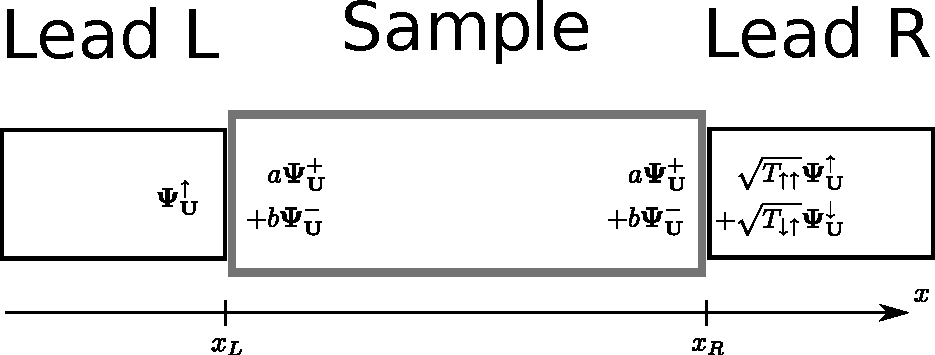
\includegraphics[width=0.8\textwidth]{adapting-pic.pdf}
    \end{center}
    \caption{Injecting one spin-up charge carrier into the system}
\end{figure}

% Since there is no dissipation in our model, and we assume that the mere
% process of injecting an electron doesn't change its spin, we can project
% the $|\uparrow>$ and $|\downarrow>$ states separately onto the wave
% function in the sample:

Since we assume that our leads are perfect semi-infinite wires, we can assume
that the wave functions are plain waves

\begin{align*}
    \mathbf{\Psi^\uparrow}   &=  e^{i p_x x} e^{i p_z z} |\uparrow> \\
    \mathbf{\Psi^\downarrow} &=  e^{i p_x x} e^{i p_z z} |\downarrow> \\
\end{align*}

and that the part of wave function in the sample which travels from left to
right is a smooth continuation of the wave function in the lead:

\begin{align}
    \mathbf{\Psi^\uparrow}(x=x_1) &=
        a\cdot e^{i p_x x_1}e^{i p_z z} \chi_N^+
        + b\cdot e^{i p_x x_1}e^{i p_z z} \chi_N^-\nonumber\\
    \mathbf{\Psi^\downarrow}(x=x_1) &=
        c\cdot e^{i p_x x_1}e^{i p_z z} \chi_N^+
        + d\cdot e^{i p_x x_1}e^{i p_z z} \chi_N^-
        \label{eq:a-n-left}
\end{align}

where $x_1$ is the location where the left lead is connected to the sample, the
interface is at $x = 0$ and the right lead is connected at $x = x_2$.
Each of these equations has two components, which allows us to determine
the coefficients $a, b, c$ and $d$ unambiguously.


We can then look at the connection to the right lead and obtain the 
elements of the transmission matrix in the $\uparrow, \downarrow$ bases:

\begin{align}
    T_{2\uparrow,1\uparrow} = \left| \left( 
        a \mathbf{\Psi^+}(x=x_2) + b  \mathbf{\Psi^-}(x=x_2)
    \right)^\dagger \cdot \mathbf{\Psi}^\uparrow(x=x_2) \right|^2\nonumber\\
    T_{2\downarrow,1\uparrow} = \left| \left( 
        a \mathbf{\Psi^+}(x=x_2) + b  \mathbf{\Psi^-}(x=x_2)
    \right)^\dagger \cdot \mathbf{\Psi}^\downarrow(x=x_2) \right|^2\nonumber\\
    T_{2\uparrow,1\downarrow} = \left| \left( 
        c \mathbf{\Psi^+}(x=x_2) + d  \mathbf{\Psi^-}(x=x_2)
    \right)^\dagger \cdot \mathbf{\Psi}^\uparrow(x=x_2) \right|^2\nonumber\\
    T_{2\downarrow,1\downarrow} = \left| \left( 
        c \mathbf{\Psi^+}(x=x_2) + d  \mathbf{\Psi^-}(x=x_2)
    \right)^\dagger \cdot \mathbf{\Psi}^\downarrow(x=x_2) \right|^2
%    \label{eq:an-right}
\end{align}

where $\mathbf{\Psi^\pm}$ are the wave functions introduced in
\ref{eq:chiral-wafe-function}. Note that these wave functions are not
normalized in the usual sense. Rather on the left of the interface ($x < 0$),
they consist of a part traveling left to right, and a part traveling right to
left. The left-to-right part is normalized the same way as
$\mathbf{\Psi^\uparrow}$
is.

Both the right-to-left part of $\mathbf{\Psi^\pm}(x < 0)$ and the whole of
$\mathbf{\Psi^\pm}(x > 0)$ are not normalized, and in magnitude generally
smaller than 1 which allows us to determine the transmission matrix elements
by looking at the amplitudes.

For comparing the analytical and numeric results, one final step is missing:
$\tso$ and $\ta$ are not the same, but it is easy to get a relation between the
two:

\begin{align}
    \tso &= \frac{\alpha\hbar}{2a}\\
    t    &= \frac{\hbar^2}{2 m a^2}\\
    \frac{\tso}{t} &= \frac{\alpha m a}{\hbar} = \frac{\ta v_F m a}{\hbar} \\
    \Rightarrow \frac{\tso}{t \ta} &= a k_F = a \sqrt{2 \pi n_{2D}}
\end{align}

where $k_F$ is the Fermi wave vector and $n_{2D} \approx 10^{11} cm^{-2}$ is
the density of states in two dimensions.

\begin{figure}
    \begin{center}
        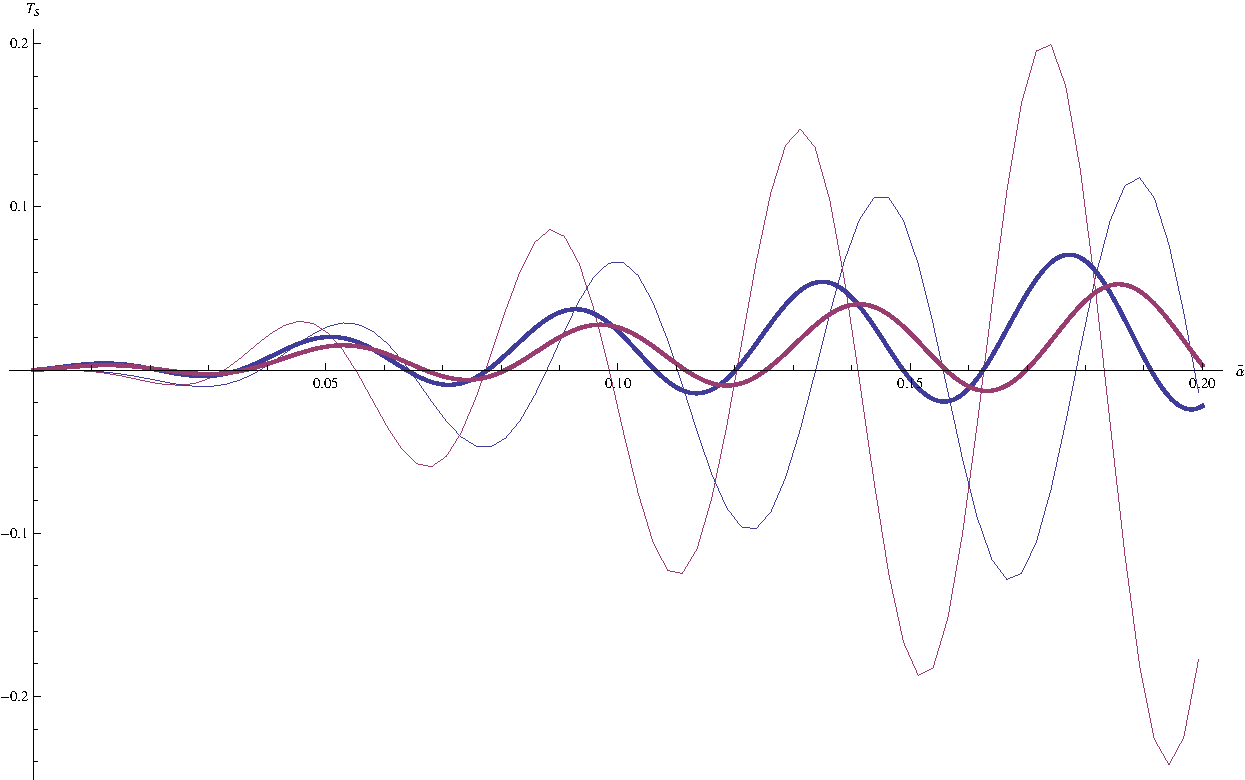
\includegraphics[width=0.8\textwidth]{comparison-over-alpha.pdf}
    \end{center}
    \caption{$T_S = T_{2\uparrow,1\uparrow} - T_{2\downarrow,1\downarrow}$ as
        a function of $\ta$. Bold curves show the results from the analytical
        calculations, thin lines from the numerical calculation.
        \textbf{Blue:} $\phi = 23^\circ$, \textbf{Red:} $\phi = 29^\circ$.
    }
    \label{fig:a-n-matching-alpha}
\end{figure}
\begin{figure}
    \begin{center}
        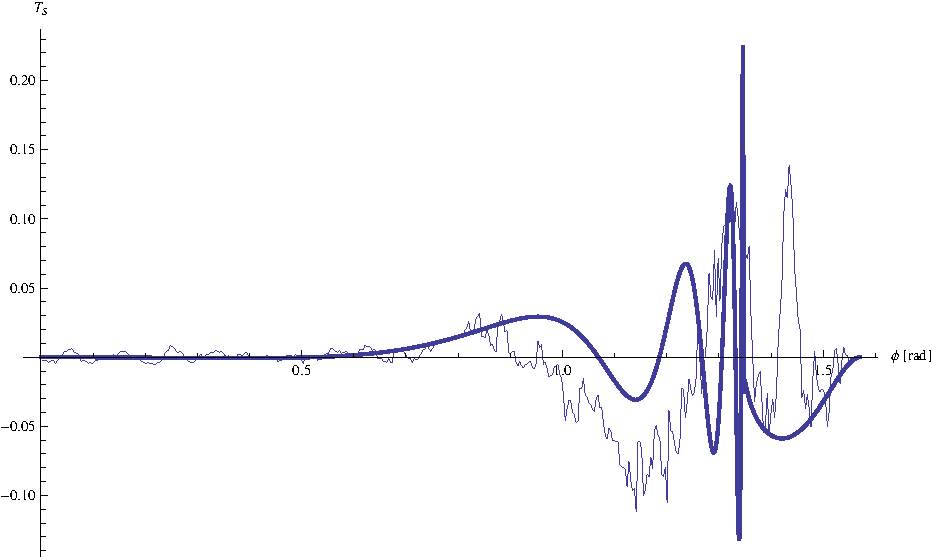
\includegraphics[width=0.8\textwidth]{comparison-over-phi.pdf}
    \end{center}
    \caption{$T_S = T_{2\uparrow,1\uparrow} - T_{2\downarrow,1\downarrow}$ as
        a function of the interface angle $\phi$ (in radians). The bold curve
            show the result from the analytical calculations, the thin line
            from the numerical calculation. $\tso = 0.02$, $E_F = 1.5t$
    }
    \label{fig:a-n-matching-phi}
\end{figure}
\begin{figure}
    \begin{center}
        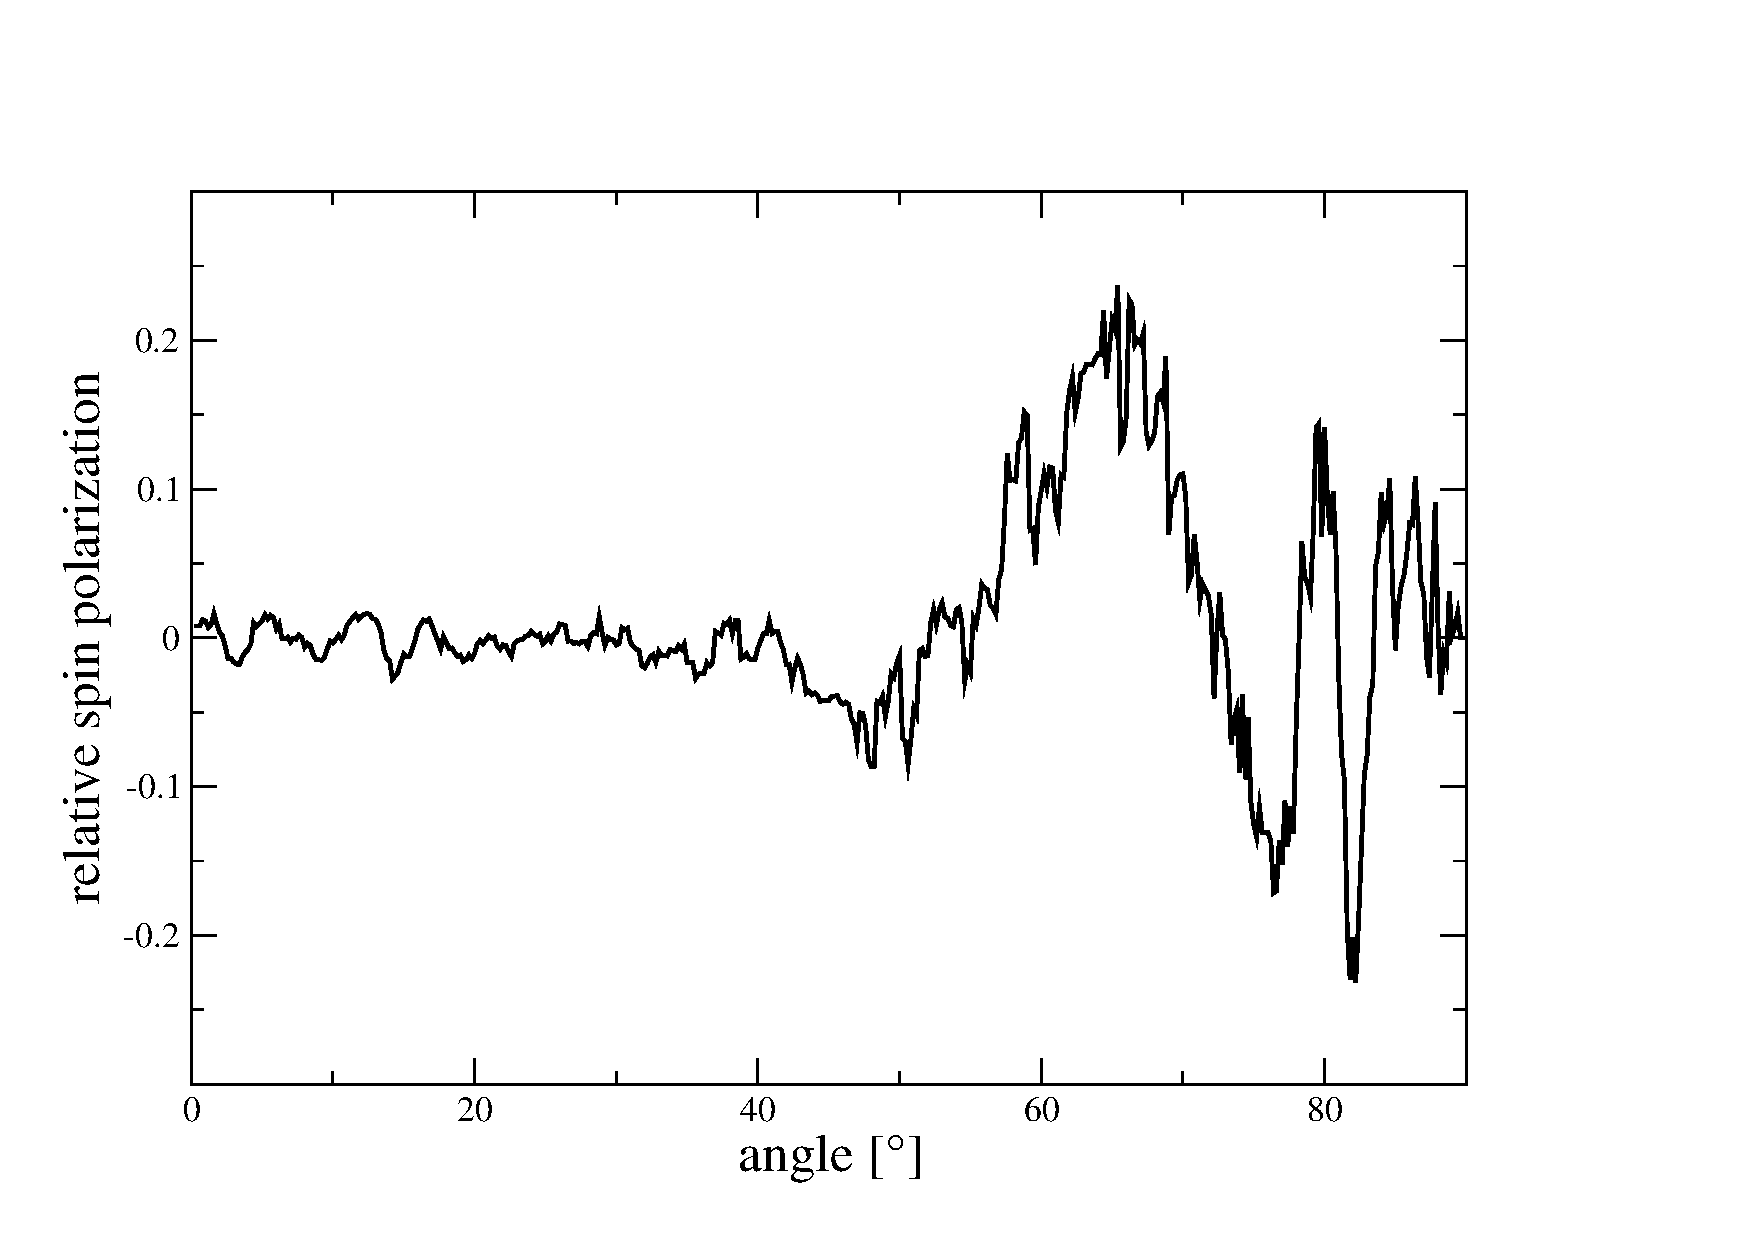
\includegraphics[width=0.8\textwidth]{relative-polarization-n-so.pdf}
    \end{center}
    \caption{$T_S^{rel} = \frac{T_{2\uparrow,1\uparrow} - T_{2\downarrow,1\downarrow}}
        {T_{2\uparrow,1\uparrow} + T_{2\downarrow,1\downarrow}}$ as
        a function of the interface angle $\phi$ (in degrees), and otherwise
        identical parameters as in fig. \ref{fig:a-n-matching-phi}.
        We observe a maximal spin polarization of about $20\%$.
        }
    \label{fig:n-so-rel}
\end{figure}

Figure \ref{fig:a-n-matching-alpha} shows the signal for two different
angles of the interface. For weak spin-orbit coupling, the theory and the
numerical results agree well, for stronger coupling both the oscillation
period and the amplitude start to disagree.

Figure \ref{fig:a-n-matching-phi} shows the effect of the interface angle
$\phi$ as for a fixed spin-orbit coupling strength. The signal from the
numerical simulation is quite noisy, because
a small variation of $\phi$ moves the steps that are used to emulate a smooth
interface.

In order to get one propagating mode in most of the sample, a rather
high Fermi energy was chosen ($E_F = 1.5t$), which means that $k_F$ is
actually quite large. The tight binding simulation only works well for small
wave vectors where the parabolic band can be well approximated with the
cosine form that the tight binding model implies. This explains why there is a
shift between the two curves in figure \ref{fig:a-n-matching-phi}.

For a rather small spin-orbit coupling strength of $\frac{\tso}{2 t a} = 0.02$
we already get a quite respectable relative spin-polarization of $20\%$.

To understand better why we don't get a very clear picture of the critical
angle the numerical results, we look at \ref{eq:a-n-left} and for a moment
ignore the global phases that the $\exp$ functions provide, and obtain a
simplified expression for $a$ and $b$.

\begin{align}
   a &= \frac{1-\sin \phi}{1 + \sin\phi} \nonumber\\
   b &= \sqrt{1-a^2}
\end{align}

Since $t_{-+}$ and $t_{+-}$ are rather small, we also neglect them, as well as
the $exp$ functions in $\mathbf{\Psi^\pm}$, which only contribute phases for
$\phi < \phi_c$. Thus we obtain approximate, 
simplified expression for our matrix elements:

\begin{align}
    T_{2\uparrow,1\uparrow}     &\approx \left|a \chi_{SO}^{+U} t_{++}
            + b \chi_{SO}^{-U} t_{--} \right|^2\\
    T_{2\downarrow,1\downarrow} &\approx \left|c \chi_{SO}^{-D} t_{--}
            + d \chi_{SO}^{+D} t_{--} \right|^2
\end{align}

where the superscript index $U$ means \emph{upper component of}, and $D$ means
\emph{lower component of}.

When $\phi$ is varied in the range of 0 to $\pi/2$, the coefficients $a, b, c,
d$ and the absolute values of the spinor components cover the range of 0 to 1.
The critical phenomena and the variation of $t_{++}$ and $t_{--}$ drown in
eight parameters which oscillate roughly with the same frequency and
magnitude, washing out a clear signature from the chiral waves.

Or speaking more in terms of physical quantities, the interface efficiently
selects waves of $-$ chirality over waves of $+$ chirality (for large angles),
but injecting and measuring the waves in the $\uparrow,\downarrow$ bases
hides a significant part of this effect.

\section{Interface Between Two Spin-Orbit Coupling Regions}

\begin{figure}[htb]
    \begin{center}
        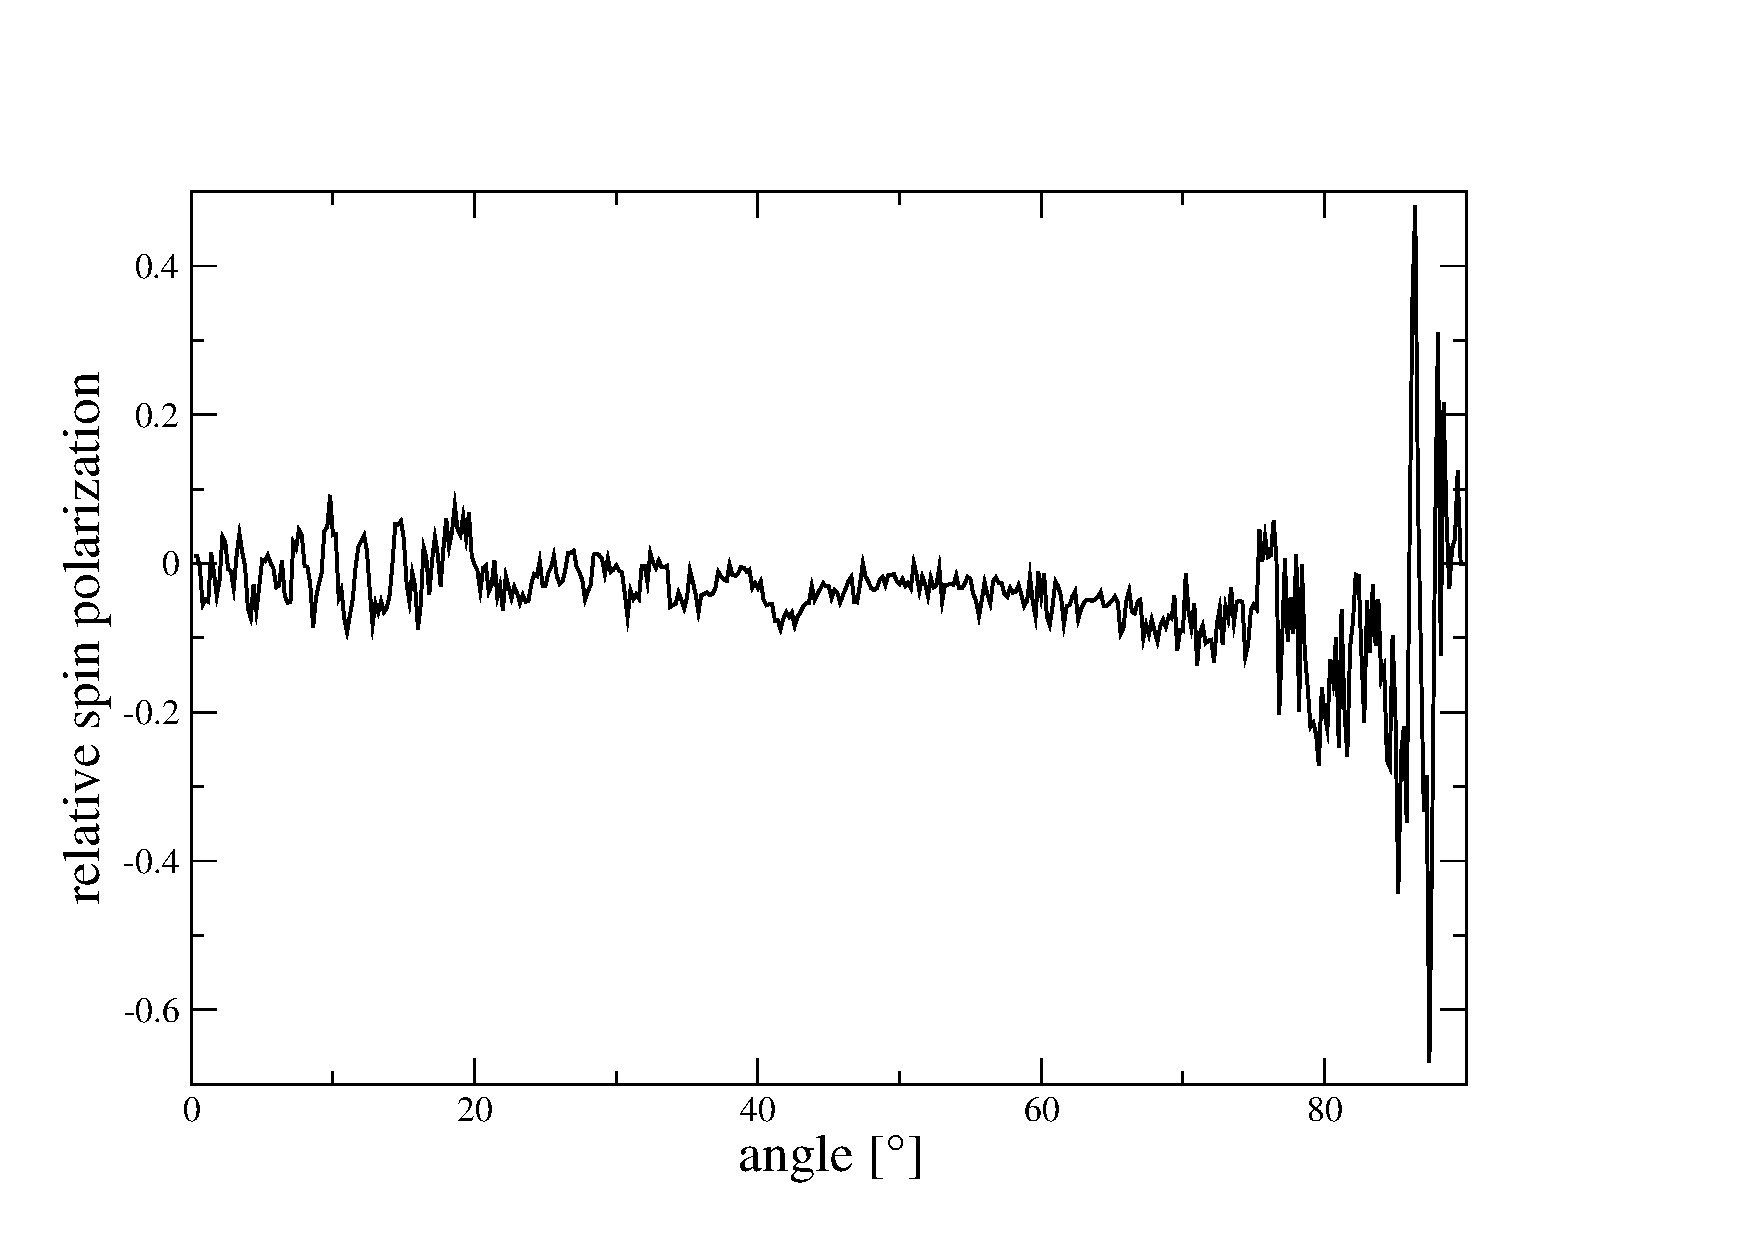
\includegraphics[width=0.8\textwidth]{relative-polarization-so-so.pdf}
    \end{center}
    \caption{$T_S^{rel} = \frac{T_{2\uparrow,1\uparrow} - T_{2\downarrow,1\downarrow}}
        {T_{2\uparrow,1\uparrow} + T_{2\downarrow,1\downarrow}}$ as
        a function of the interface angle $\phi$ (in degrees), for an
        interface of two non-zero spin-orbit coupling regions. $t_{SO,B} =
        \frac{0.1}{2 a t}$, $t_{SO,A} = 0.5 t_{SO,B}$. As in the case of
        a N and SO region, we can observe a spin polarization of about $20\%$,
          with additional peaks going up to about $40\%$.
        ($150 \times 150$ sample of $100~nm \times 100~nm$ at $E_F = 2 t$)
        }
    \label{fig:n-so-rel}
\end{figure}

When a sample contains a 2-dimensional electron gas with Rashba spin-orbit
coupling, it is very hard to create a region without any spin-orbit coupling.
While it is hard to switch it off entirely, it is quite possible to tune the
strength of an individual region by using a gate electrode on top of the
sample to apply an electric field.

Figure \ref{fig:n-so-rel} shows the relative spin polarization as a function
of the interface angle $\phi$, for $\ta_B = 2 \ta_A$. Again a spin
polarization of $20\%$ can be observed, with some few spikes going up as high
as $40\%$ (but with stronger SO interaction on the right-hand side than in the
case of the N-SO interface).

\begin{figure}[htb]
    \begin{center}
        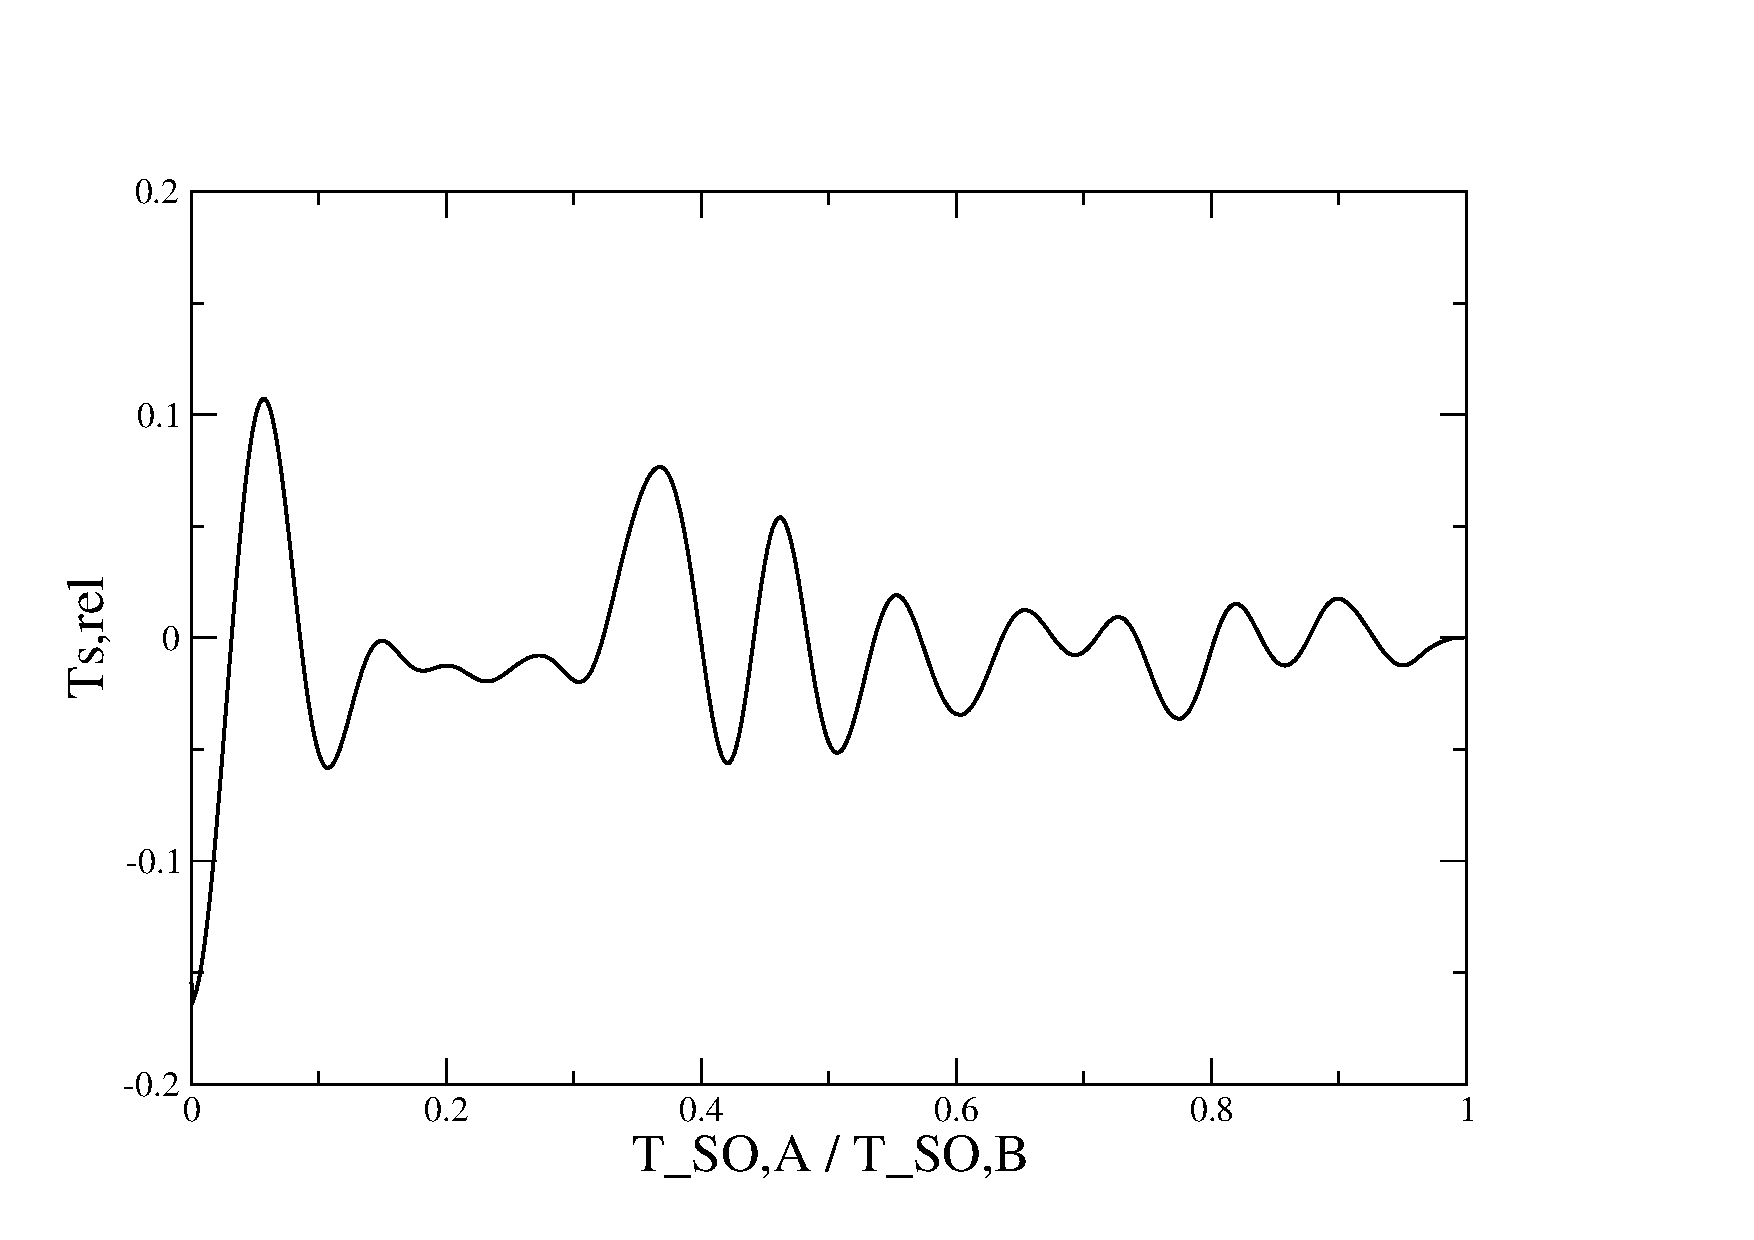
\includegraphics[width=0.7\textwidth]{polarization-so-so-rel.pdf}
    \end{center}
    \caption{Relative spin polarization $T_s^{rel}$ as function of $q 
=\frac{\ta_A}{\ta_B}$ (ratio of spin-orbit coupling strength) for a fixed
    $\phi=80^\circ$ and $\tso{}_B = 0.1$.}
    \label{fig:pol-so-so-rel}
\end{figure}

To find out how much the spin polarization depends on the relative strength of
spin-orbit coupling in the two regimes, we plot $T_S^{rel}$ over $q
=\frac{\ta_A}{\ta_B}$ for a fixed $\ta_B$ (see fig.~\ref{fig:pol-so-so-rel}).

You can see that for $q = 0$ the spin polarization is about $15\%$, and shows
the usual spin precession effects that come with changing $\tso$. Additionally
the envelope function decreases for $q \mapsto 1$, because the regions become
similar and thus the effect of the interface less pronounced.

%For $\phi > \phi_c$, the wave $\exp{i p_x^+ x}\exp{i p_z z} t_{++}\chi_{SO}^+$
%does not propagate, because $p_x^+$ is imaginary. That means that the relative
%spin polarization caused by the $\mathbf{\Psi^+}$ wave
%is  the difference of squares of the components of $\chi_{SO}^-$
%(see equation \ref{eq:chi-so-pm} for the explicit form of $\chi_{SO}^-$).

%\begin{align}
%    |T_s^{\textnormal{rel}}| &= \left| \frac{T_{2\uparrow,1\uparrow} -
%        T_{2\downarrow,1\downarrow}}{T_{2\uparrow,1\uparrow}
%            +T_{2\downarrow,1\downarrow}} \right| \nonumber \\
%        &= \frac{\left| |p^+_{SO} - p_{x,SO}^+|^2 -
%    p_z^2\right|}{|p_{SO}^+ - p_{x,SO}^+|^2 + p_z^2} \qquad \textnormal{ for }
%    \phi > \phi_c
%\end{align}
%
%\begin{figure}
%    \begin{center}
%        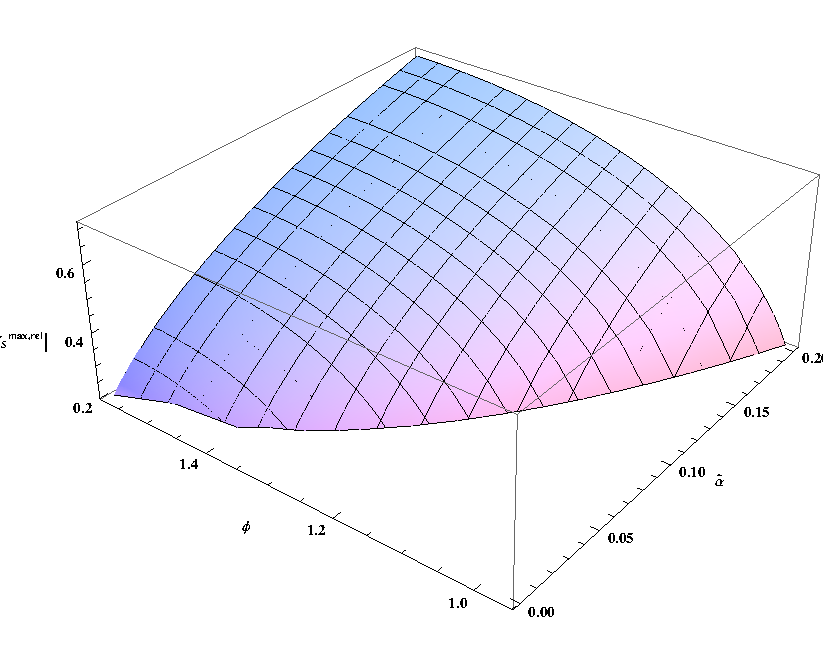
\includegraphics[width=0.8\textwidth]{max-spin-polarization.pdf}
%    \end{center}
%    \caption{Relative spin polarization above the critical angle
%        $\phi_c$ as caused by the incident wave with $+$ chirality}
%\end{figure}

% vim: ts=4 sw=4 expandtab spell spelllang=en_us tw=78



\bibliography{bib}

\end{document}

% vim: ts=4 sw=4 expandtab spell spelllang=en_us tw=78
